\documentclass[a4paper, twoside,openright]{report}

\usepackage[table]{xcolor}
\usepackage{listings}
\usepackage{xcolor}
\usepackage[newfloat]{minted}
\usepackage{caption}
\usepackage{soul}
\definecolor{inlineBG}{HTML}{F3F3F3} \sethlcolor{inlineBG}
\let\OldTexttt\texttt
\renewcommand{\hltexttt}[1]{\sethlcolor{inlineBG}{\ttfamily\hl{\mbox{#1}}}}

\usepackage{tikz}
\usepackage{algorithm}
\usepackage[noend]{algpseudocode}
\usepackage{capt-of}
%\usepackage{float}
\usepackage{comment}
\usepackage[a4paper,top=3cm,bottom=3cm,left=3cm,right=3cm]{geometry}
\usepackage[fontsize=15pt]{scrextend}
\usepackage[english]{babel}
\usepackage[fixlanguage]{babelbib}
\usepackage[utf8]{inputenc}
\usepackage[T1]{fontenc}
\usepackage{lipsum}
\usepackage{rotating}
\usepackage{fancyhdr}
\usepackage{amssymb}
\usepackage{amsmath}
\usepackage{amsthm}
\usepackage{graphicx}
\usepackage[dvipsnames]{xcolor}
\usepackage{listings}
\usepackage{hyperref}
\usepackage[normalem]{ulem}
\usepackage{bbm}

\pagestyle{fancy}
\fancyhf{}
\lhead{\rightmark}
\rhead{\textbf{\thepage}}
\fancyfoot{}
\setlength{\headheight}{12.5pt}

\fancypagestyle{plain}{
  \fancyfoot{}
  \fancyhead{}
  \renewcommand{\headrulewidth}{0pt}
}

\lstdefinestyle{codeStyle}{
    commentstyle=\color{teal},
    keywordstyle=\color{Magenta},
    numberstyle=\tiny\color{gray},
    stringstyle=\color{violet},
    basicstyle=\ttfamily\footnotesize,
    breakatwhitespace=false,
    breaklines=true,
    captionpos=b,
    keepspaces=true,
    numbers=left,
    numbersep=5pt,
    showspaces=false,
    showstringspaces=false,
    showtabs=false,
    tabsize=2
} \lstset{style=codeStyle}

\lstdefinestyle{longBlock}{
    commentstyle=\color{teal},
    keywordstyle=\color{Magenta},
    numberstyle=\tiny\color{gray},
    stringstyle=\color{violet},
    basicstyle=\ttfamily\scriptsize,
    breakatwhitespace=false,
    breaklines=true,
    captionpos=b,
    keepspaces=true,
    numbers=left,
    numbersep=5pt,                  
    showspaces=false,
    showstringspaces=false,
    showtabs=false,
    tabsize=2
} \lstset{style=codeStyle}

\lstset{aboveskip=20pt,belowskip=20pt}

\hypersetup{
    colorlinks,
    linkcolor=CornflowerBlue,
    citecolor=CornflowerBlue
}

\newtheorem{definition}{Definition}[section]
\newtheorem{theorem}{Theorem}[section]
\providecommand*\definitionautorefname{Definition}
\providecommand*\theoremautorefname{Theorem}
\providecommand*{\listingautorefname}{Listing}
\providecommand*\lstnumberautorefname{Line}

\raggedbottom

\begin{document}
\pagenumbering{arabic}

\begin{titlepage}
\begin{figure}[!htb]
    \centering
    \includegraphics[keepaspectratio=true,scale=0.5]{contents/Frontpage/cherubinFrontespizio.eps}
\end{figure}

\begin{center}
    \LARGE{UNIVERSITÀ DI PISA}
    \vspace{5mm}
    \\ \large{DEPARTMENT OF COMPUTER SCIENCE}
    \vspace{5mm}
    \\ \large{Master Degree in Computer Science} \vspace{5mm}
    \\ \large{Artificial Intelligence curriculum}
\end{center}

\vspace{20mm}
\begin{center}
    {\large{\bf Federated Echo State Networks \\ \vspace{3mm} for Stress Prediction in the Automotive Use Case}}
\end{center}
\vspace{30mm}

\begin{minipage}[t]{0.47\textwidth}
	{\large{Supervisors:}{
	\normalsize \vspace{3mm}
	\bf \\ \large{Prof. Davide Bacciu} \normalsize \vspace{3mm}
	\bf \\ \large{Prof. Iraklis Varlamis}
	\normalsize \vspace{3mm}
	\bf \\ \large{Dr. Valerio De Caro}
	}}
\end{minipage}
\hfill
\begin{minipage}[t]{0.47\textwidth}\raggedleft
	{\large{Candidate:}{\normalsize\vspace{3mm} \bf\\ \large{Antonio Di Mauro}}}
\end{minipage}

\vspace{12mm}
\hrulefill
\\\centering{\large{ACADEMIC YEAR 2021/2022}}

\end{titlepage}

\tableofcontents

\listoffigures

\listoftables

\lstlistoflistings

\listofalgorithms

\chapter{Introduction}

Recent years have witnessed the rapid development of the Internet of Things (IoT) which provides ubiquitous sensing and computing capabilities to connect a broad range of things to the Internet \cite{lin2017survey}. To obtain insights on the data generated from ubiquitous IoT devices, Artificial Intelligence (AI) techniques such as Deep Learning (DL) have been widely exploited to train data models for enabling intelligent IoT applications such as smart healthcare, smart transportation and smart city \cite{mohammadi2018enabling}. \\

Traditionally, AI functions are placed in a cloud server or a data center for data learning and modeling \cite{sun2019application}, which incurs critical limitations given the huge amount of data from IoT sources. According to Cisco, there are nearly 850 ZB of data generated by all people, machines and things at the network edge by 2021. In sharp contrast, the global data center traffic is presumed reaching 20.6 ZB in 2021 \cite{cisco}. With such a tremendous growth of
IoT data at the network edge, in line with the growth in the number of devices (Fig. \ref{fig:growth}), centralizing the computation on the remote servers may be infeasible due to the required network resources and the incurred latency.

\begin{center}
\begin{minipage}[c]{\textwidth}
    \centering
    \includegraphics[width=0.8\textwidth]{contents/Chapter1/growth.png}
    \captionof{figure}{Global device and connection growth \cite{cisco2}}
    \label{fig:growth}
\end{minipage}
\end{center}

Furthermore, the use of third-party servers for AI training also raises privacy concerns, as training data may contain sensitive information such as user addresses or personal preferences \cite{granjal2015security}. It is thus highly necessary for developing innovative AI approaches to realize efficient and privacy-enhanced intelligent IoT networks and applications. \\

%\section{EU H2020 TEACHING Project}

Concurrently, both industry and society are experiencing the transformational impact of the autonomous systems revolution, empowered by automation capabilities offered by Artificial Intelligence (AI). Cyber-physical Systems of Systems (CPSoS) define a multi-faceted and dynamic environment where autonomy is fundamental to govern the complexity of interactions between the virtual and physical worlds with minimal human intervention. However, even when the most advanced degree of autonomy is exercised, the human is a variable which cannot be left out of the CPSoS equation, particularly in safety critical scenarios like autonomous transportation \cite{teachingUnipi}. \\

In this context, the TEACHING project\footnote{\url{https://teaching-h2020.eu/}} (i.e., a computing Toolkit for building Efficient Autonomous appliCations leveraging Humanistic INtelliGence) is an EU-funded project that puts forward a vision of humans at the center of autonomous CPSoS. Embracing the concept of Humanistic Intelligence, it pursues a vision where the CPSoS adapts itself by means of human feedback, achieving a mutual empowerment towards a shared goal. \\

The objective of the Project is the design, development and deployment of autonomous, adaptive and dependable CPSoS applications, allowing them to exploit a sustainable human feedback to drive, optimize and personalize the provisioning of their services. \\

This Work was done under the Human State Monitoring task of the TEACHING project, and aims to develop an efficient learning model for predicting the stress conditions of a human driver from physiological data. Being such data inherently distributed and privacy-constrained, the further challenge that we addressed was to perform the learning in a federated environment. \\

Specifically, this Work tries to improve the State of the Art (SOTA) performances of an Echo State Network (ESN) used for the prediction of the stress value of a human driving car, which acts as a proxy for adapting the driving profile. The final model is analyzed in a FL scenario to compare different FL algorithms and comparing them with SOTA performances. \\

In Chapter \ref{chapter:background} are analyzed the theoretical aspects concerning the ESN model, FL algorithms and FL applied to ESNs. In Chapter \ref{chapter:fedcurv} is explained the specific implementation of the FL algorithm FedCurv used on ESNs. In Chapter \ref{chapter:disc} is discussed the novel approach of discriminating among anomalous/not anomalous client in the federated setting. Chapter \ref{chapter:dataset} is focused on the preprocessing of the WESAD Dataset\footnote{\url{https://archive.ics.uci.edu/ml/datasets/WESAD+\%28Wearable+Stress+and+Affect+Detection\%29}} used for the experiments that are explained in Chapter \ref{chapter:experiments}. The conclusions and future works are discussed in Chapter \ref{chapter:conclusions}.

\chapter{Background}\label{chapter:background}

In this Chapter are analyzed theoretical aspects behind Reservoir Computing (RC), with a focus on Echo State Networks (ESNs). Next, we will address Federated Learning (FL) along with two different FL algorithms: \texttt{FedAvg} and \texttt{FedCurv}. Finally, we will discuss the specific aspect of FL applied to ESNs.

\section{Reservoir Computing and Echo State Networks}

Artificial Recurrent Neural Networks (RNNs) represent a large and varied class of computational models that are designed in analogy with biological brain modules. In an RNN numerous abstract neurons (also called units or processing elements) are interconnected by likewise abstracted synaptic connections (or links), which enable activations to propagate through the network. The characteristic feature of RNNs that distinguishes them from the feedforward neural networks is that the connection topology possesses feedback loops. Such loops enable the RNNs to may develop a self-sustained temporal activation dynamics along its recurrent connection pathways, even in the absence of input. Mathematically, RNNs enrich feedforward neural networks by introducing the temporal component in the equation, making it a dynamical system modelled by its corresponding differential equation. If driven by an input signal, an RNN preserves in its internal state a nonlinear transformation of the input history, in other words, it has a dynamical memory, and is able to process temporal context information \cite{lukovsevivcius2009reservoir}. \\

The main shortcoming of RNNs is that they are difficult to train by gradient-descent-based methods, which aim at iteratively reducing the training error. The reasons behind such difficulty are twofold. First, gradual change of network parameters during learning drives the network dynamics through bifurcations \cite{doya1992bifurcations}. At such points, the gradient information degenerates and may become ill-defined. As a consequence, convergence cannot be guaranteed. Second, computing the gradient of the error requires unfolding the network over time, which increases the computational cost of the learning algorithm and may make it unfeasible depending on the size of the model and the supporting hardware. Another shortcoming is represented by the difficulty of learning long-term dependencies, since the necessary gradient information exponentially dissolves over time \cite{bengio1994learning}. Long Short-Term Memory (LSTM) networks represents a possible solution \cite{gers2000learning}. However, besides the difficulty of handling its corresponding learning algorithms \cite{lukovsevivcius2009reservoir}, this model still falls back in the shortcoming described above. \\

In this situation of slow and difficult progress, in 2001 a fundamentally new approach to RNN design and training was proposed by Wolfgang Maass under the name of Liquid State Machines \cite{maass2002real} and by Herbert Jaeger under the name of Echo State Networks (ESNs) \cite{jaeger2001echo}. This approach is often referred to as Reservoir Computing (RC). The RC paradigm avoids the shortcomings of gradient-descent RNN training stated above, by setting up RNNs in the following way:

\begin{itemize}
    \item A Recurrent Neural Network is \textit{randomly} created and remains unchanged during training. This RNN is called the \textit{reservoir}. It is passively excited by the input signal and maintains in its state a nonlinear transformation of the input history.
    
    \item The desired output signal is generated as a linear combination of the neuron’s signals from the input-excited reservoir. This linear combination, named \textit{readout}, is obtained by linear regression, using the teacher signal as a target.
\end{itemize}

\subsection{Echo State Network Formalization}

Let a \textit{problem} or a \textit{task} in our context of machine learning be defined as a problem of learning a functional relation between a given input $\textbf{u}(t) \in \mathbb{R}^{N_u}$ and a desired output $\textbf{y}_{target}(t) \in \mathbb{R}^{N_y}$, where $t=1,\dots ,T$, and $T$ is the number of data points in the training \textit{dataset} $\{(\textbf{u}(t), \textbf{y}_{target}(t))\}$. In a \textit{temporal task} the function to be learned depends on the history of the input, so the expansion function has memory: $\textbf{x}(t)=x(\dots, \textbf{u}(t-1), \textbf{u}(t))$, i.e., it is an expansion of the current input and its (potentially infinite) history. Since this function has an unbounded number of parameters, practical implementations often take an alternative, recursive, definition:

\begin{equation}\label{eq:temporal_task}
    \textbf{x}(t)=x(\textbf{x}(t-1), \textbf{u}(t)).
\end{equation}

The type of Recurrent Neural Networks that we will consider in this Work is a straightforward implementation of Eq. \ref{eq:temporal_task} where a nonlinear expansion with memory here leads to a \textit{state vector} of the form:

\begin{equation}\label{eq:reservoir_state}
    \textbf{x}(t)=f(\textbf{W}_{in}\textbf{u}(t)+\widehat{\textbf{W}}\textbf{x}(t-1)), t=1,\dots , T.
\end{equation}

where $\textbf{x}(t) \in \mathbb{R}^{N_x}$ is a vector of reservoir neuron activations at a time step $t$, $f(\cdot)$ is the neuron activation function, usually the $tanh(\cdot)$, $\textbf{W}_{in} \in \mathbb{R}^{N_x \times N_u}$ is the input weight matrix, and $\widehat{\textbf{W}} \in \mathbb{R}^{N_x \times N_x}$ is a weight matrix of internal network connections. The network is usually started with the initial state $\textbf{x}(0)=0$.
The \textit{readout} of the network is implemented in this way:

\begin{equation}\label{eq:readout}
    \textbf{y}(t)=f_{out}(\textbf{W}\textbf{x}(\textbf{u}(t)))
\end{equation}

where $f_{out}(\cdot)$ is a nonlinear function (e.g., a sigmoid applied element-wise), $\textbf{W} \in \mathbb{R}^{N_y \times N_x}$ are the trained output weights. \\

Echo State Networks \cite{jaeger2007echo} represent one of the two pioneering reservoir computing methods. The approach is based on the observation that if a random RNN possesses certain algebraic properties, training only a linear readout from it is often sufficient to achieve excellent performance in practical applications. The untrained layer of the ESN is called a \textit{dynamic reservoir}, and the resulting states $\textbf{x}(t)$ are termed \textit{echoes} of its input history \cite{jaeger2001echo}, this is where Reservoir Computing draws its name from. \\

\begin{center}
\begin{minipage}[c]{\textwidth}
    \centering
    \includegraphics[width=0.6\textwidth]{contents/Chapter2/esn-arch.png}
    \captionof{figure}{Architecture of an ESN. The input signal $\textbf{u}(t)$ is fed to the recurrent reservoir. Then, a state $\textbf{x}(t)$ is extracted from the reservoir, from which an output $\textbf{y}(t)$ is computed \cite{bacciu2021federated}}
    \label{fig:esn_arch}
\end{minipage}
\end{center}

A fundamental constraint of the ESNs is that we must ensure the stability of the dynamical system. Such constraint is satisfied by the \textit{Echo State Property} (ESP) \cite{jaeger2001echo} (Def. \ref{def:esp}). Apply the sufficient condition (Theorem \ref{thm:suff_cond_esp}) for the ESP is fine in theory, but often impractical because it is too strong. Usually, the necessary condition (Theorem \ref{thm:nec_cond_esp}) is used as an easy way for initialization of the reservoir. \\

The necessary condition states that the effect of a previous state $\textbf{x}(t)$ and a previous input $\textbf{u}(t)$ on a future state $\textbf{u}(t+k)$ should vanish gradually as time passes (i.e. $k\rightarrow\infty$), and not persist or even get amplified \cite{lukovsevivcius2009reservoir}. For most practical purposes, the ESP is assured if the reservoir weight matrix $\widehat{\textbf{W}}$ is scaled so that its spectral radius $\rho(\widehat{\textbf{W}})$ (i.e., the largest absolute eigenvalue) satisfies $\rho(\widehat{\textbf{W}})<1$ \cite{jaeger2001echo} or, using
another term, $\widehat{\textbf{W}}$ is \textit{contractive}. Practically, the initialization of $\widehat{W}$ is made in the following way:

\begin{equation}
    \widehat{\textbf{W}} \leftarrow \widehat{\textbf{W}} \frac{\rho_{desired}}{\rho(\widehat{\textbf{W}})}
\end{equation}

where $\rho_{desired} < 1$. Also the $\textbf{W}_{in}$ matrix could be initialized in the following way:

\begin{equation}
    \textbf{W}_{in} \leftarrow \omega_{in}\textbf{W}_{in}
\end{equation}

where $\omega_{in}$ is the \textit{input scaling} parameter that makes $\textbf{W}_{in}$ values falling in the interval $[-\omega_{in}, \omega_{in}]$ if the elements of $\textbf{W}_{in}$ are generated randomly from a uniform distribution on the interval $[-1,1]$. The spectral radius $\rho(\widehat{\textbf{W}})$ and the input scaling $\omega_{in}$ are key hyper-parameters of the reservoir initialization. \\


\begin{definition}[Reservoir State Transition Function]\label{def:rstf}
Given $N_u$ the input dimension and $N_x$ the number of reservoir neurons. The reservoir is a discrete-time input-driven dynamical system, and its dynamics are driven by the State Transition Function:

\begin{equation}\nonumber
    F:\mathbb{R}^{N_u} \times \mathbb{R}^{N_x} \rightarrow \mathbb{R}^{N_x}
\end{equation}

\begin{equation}
    \textbf{x}(t)=F(\textbf{u}(t), \textbf{x}(t-1))
\end{equation}

where $F$ takes an input and a state and returns a new state. The final state after seeing an entire input sequence s, given the initial state, is given by the iterative version of the State Transition Function:

\begin{equation}\nonumber
    \widehat{F}:(\mathbb{R}^{N_u})^* \times \mathbb{R}^{N_x} \rightarrow \mathbb{R}^{N_x}
\end{equation}

\begin{equation}
    \widehat{F}(s,x_0)=\left\{\begin{matrix}x_0 & \textup{if s=[ ]}\\F(x(t), \widehat{F}([x(1),\dots, x(t-1)],x_0)) & \textup{if s=[x(1),\dots, x(t)]}
\end{matrix}\right.
\end{equation} \\
\end{definition}


\begin{definition}[Echo State Property (ESP)]\label{def:esp}
Given $N_u$ the input dimension, $N_x$ the number of reservoir neurons and the State Transition Function $\widehat{F}$ (Def. \ref{def:rstf}). An ESN satisfies the ESP whenever:

\begin{equation}\nonumber
    \forall s \in (\mathbb{R}^{N_u})^N, \forall x_0,z_0 \in \mathbb{R}^{N_x}:
\end{equation}

\begin{equation}
    \left\| \widehat{F}(s, x_0)-\widehat{F}(s, z_0) \right\| \rightarrow 0, \text{\quad as\quad} N \rightarrow \infty
\end{equation}

briefly, given the input sequence and two initial states, the distance between the final stages goes to 0 with the length of the input. \\
\end{definition}


\begin{theorem}[Sufficient Condition for the ESP]\label{thm:suff_cond_esp}
If the maximum singular value of $\widehat{W}$ is less than 1 the ESN satisfies the ESP for any possible input.

\begin{equation}
    \sigma_{max}(\widehat{W})=\left\| \widehat{W} \right\|_2 < 1
\end{equation}

in other therms, there is a contractive dynamics for every input. \\
\end{theorem}


\begin{theorem}[Necessary Condition for the ESP]\label{thm:nec_cond_esp}
If the spectral radius of $\widehat{W}$ is not smaller than 1 the ESN does not satisfies the ESP.

\begin{equation}
    \rho(\widehat{W})=\max(abs(eig(\widehat{W})) < 1
\end{equation}

in other therms, there is a globally asymptotically stable dynamics around the 0 state. \\
\end{theorem}


ESNs (Def. \ref{def:esn}) standardly computes the reservoir states as in Eq. \ref{eq:reservoir_state}, where the nonlinear function $f(\cdot)$ is a sigmoid, usually the $tanh(\cdot)$ function. Leaky integrator neuron models represent another frequent option for ESNs (Def. \ref{def:liesn}), and is the one used in this Work and named Li-ESNs. \\

\begin{definition}[ESN]\label{def:esn}
Given $N_u$ the input dimension, $N_x$ the number of reservoir neurons, $N_y$ the output dimension and $\textbf{x}(0)=0$, the ESN at each time step $t \in \{1,\dots, T\}$ computes the state vector $\textbf{x}(t) \in \mathbb{R}^{N_x}$ for a given input signal $\textbf{u}(t) \in \mathbb{R}^{N_u}$ as:

\begin{equation}\nonumber
    \textbf{x}(t)=\tanh(\textbf{W}_{in}\textbf{u}(t)+\widehat{\textbf{W}}\textbf{x}(t-1)).
\end{equation}

where $\textbf{W}_{in} \in \mathbb{R}^{N_x \times N_u}$ and $\widehat{\textbf{W}} \in \mathbb{R}^{N_x \times N_x}$ are fixed and untrained. The readout of the network $\textbf{y}(t) \in \mathbb{R}^{N_y}$ is computed as:

\begin{equation}\nonumber
    \textbf{y}(t)=sigmoid(\textbf{W}x(\textbf{u}(t)))
\end{equation}

where $\textbf{W} \in \mathbb{R}^{N_y \times N_x}$ is trainable. \\\\
\end{definition}



\begin{definition}[Li-ESN]\label{def:liesn}
Given $N_u$ the input dimension, $N_x$ the number of reservoir neurons, $N_y$ the output dimension, $\textbf{x}(0)=0$ and $\alpha \in \mathbb{R}$ the leaking rate $(0<\alpha\leq1)$, the Li-ESN at each time step $t \in \{1,\dots, T\}$ computes the state vector $\textbf{x}(t) \in \mathbb{R}^{N_x}$ for a given input signal $\textbf{u}(t) \in \mathbb{R}^{N_u}$ as:

\begin{equation}\nonumber
    \textbf{x}(t)=(1-\alpha)\textbf{x}(t-1)+\alpha \tanh(\textbf{W}_{in}\textbf{u}(t)+\widehat{\textbf{W}}\textbf{x}(t-1)).
\end{equation}

where $\textbf{W}_{in} \in \mathbb{R}^{N_x \times N_u}$ and $\widehat{\textbf{W}} \in \mathbb{R}^{N_x \times N_x}$are fixed and untrained. The readout of the network $\textbf{y}(t) \in \mathbb{R}^{N_y}$ is computed as:

\begin{equation}\nonumber
    \textbf{y}(t)=sigmoid(\textbf{W}x(\textbf{u}(t)))
\end{equation}

where $\textbf{W} \in \mathbb{R}^{N_y \times N_x}$ is trainable.
\end{definition}


\section{Federated Learning}

Nowadays phones and tablets are the primary computing devices for many people \cite{poushter2016smartphone}\cite{anderson2015technology}. The powerful sensors on these devices (including cameras, microphones, and GPS), combined with the fact they are frequently carried, means they have access to an unprecedented amount of data, much of it private in nature. Models learned on such data hold the promise of greatly improving usability by powering more intelligent applications, but the sensitive nature of the data means there are risks and responsibilities to storing it in a centralized location. \\

Recently, the concept of Federated Learning (FL) has been proposed for building intelligent and privacy-enhanced IoT systems. Technically, FL is a distributed collaborative AI approach that allows for data training by coordinating multiple devices with a central server without sharing actual datasets \cite{konevcny2016federated}. \\

For instance, multiple IoT devices can act as workers to communicate with an aggregator (e.g. a server) for performing neural network training in intelligent IoT networks. More specifically, the aggregator first initiates a global model with
learning parameters. Each worker downloads the current model from the aggregator, computes its model update (e.g. Stochastic Gradient Descent) by using its local dataset, and sends the computed local update back to the aggregator. \\

Then, the aggregator combines all local model updates and constructs a new improved global model. By using the computing power of distributed workers, the aggregator can enhance the training quality while minimizing user privacy leakage. \\

Finally, the local workers download the global update from the aggregator, and compute their next local update until the global training is complete \cite{nguyen2021federated}.


\subsection{Federated Averaging}

Google researchers, in 2017, proposed \textit{FederatedAveraging} (or \texttt{FedAvg}) \cite{mcmahan2017communication} algorithm that makes as contributions 1) the identification of the problem of training on decentralized data from mobile devices while complying to privacy constraints as an important research direction; 2) the selection of a straightforward and practical algorithm that can be applied to this setting; and 3) an extensive empirical evaluation of the proposed approach. \texttt{FedAvg} is a general implementation of \texttt{FedSGD} and more concretely, it combines local stochastic gradient descent (SGD) on each client with a server that performs model averaging. It is robust to unbalanced and non-IID data distributions, and can reduce the rounds of communication needed to train a deep network on decentralized data by orders of magnitude. \\

It addresses the key issues of client availability and unbalanced and non-IID data. It assumes also a synchronous update scheme that proceeds in rounds of communication. There is a fixed set of $K$ clients, each with a fixed local dataset. At the beginning of each round, a random fraction $C$ of clients is selected, and the server sends the current global algorithm state to each of these clients (e.g., the current model parameters). Each selected client then performs local computation based on the global state and its local dataset, and sends an update to the server. The server then applies these updates to its global state, and the process repeats. \\

\begin{figure}[H]\label{fig:fedavg}
\centering
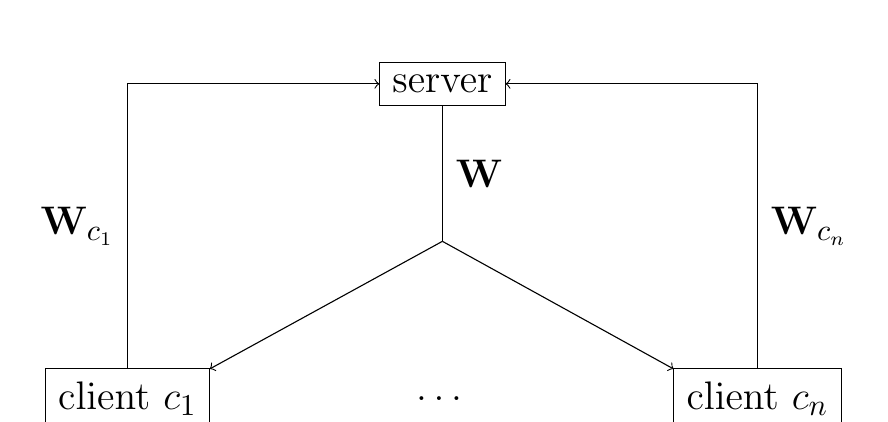
\begin{tikzpicture}[scale=2]
  \draw[line width=0pt]
    (2,2) node[draw] (s) {server}
    (0,0)  node[draw] (c1) {client $c_1$}
    (4,0)  node[draw] (cn) {client $c_n$}
    (2,0)  node[draw=none] (d) {$\dots$};

  \draw[->] (2,1)--(c1.north east);
  \draw[->] (2,1)--(cn.north west);
  \draw (2,1)-- node[right] {\textbf{W}} (s);
  \draw[->] (c1.north)-- node[left] {$\textbf{W}_{c_1}$} (0,2)--(s.west);
  \draw[->] (cn.north)-- node[right] {$\textbf{W}_{c_n}$} (4,2)--(s.east);
\end{tikzpicture}
\caption{Federated Averaging Scheme. Each client $c$ sends their local matrix $\textbf{W}_c$ to the server. After the aggregation of the models is performed in the form of a weighted average, the server sends back the same matrix $\textbf{W}$ to all clients \cite{bacciu2021federated}.}
\end{figure}

The algorithm considered is applicable to any finite-sum objective of the form:

\begin{equation}\label{eq:fedavg_obj}
    \min_{w\in\mathbb{R}^d}f(w) \textup{\quad where\quad} f(w)=\frac{1}{n}\sum_{i=1}^{n}f_i(w).
\end{equation}

For a machine learning problem, we typically take $f_i(w)=\ell(x_i,y_i;w)$, that is, the loss of the prediction on example $(x_i,y_i)$ made with model parameters $w$. We assume there are $K$ clients over which the data is partitioned, with $\mathcal{P}_k$ the set of indexes of data points on client $k$, with $n_k=\left| \mathcal{P}_k \right|$. Thus, we can rewrite the objective in Eq. \ref{eq:fedavg_obj} as:

\begin{equation}
    f(w)=\sum_{i=1}^{K}\frac{n_k}{n}F_k(w) \text{\quad where\quad} F_k(w)=\frac{1}{n_k}\sum_{i\in\mathcal{P}_k}f_i(w).
\end{equation}

If the partition $\mathcal{P}_k$ was formed by distributing the training examples over the clients uniformly at random, then we would have $\mathbb{E}_{\mathcal{P}_k}\left[ F_k(w) \right]=f(w)$, where the expectation is over the set of examples assigned to a fixed client $k$. This is the IID assumption typically made by distributed optimization algorithms; \texttt{FedAvg} refers to the case where this does not hold (that is, $F_k$ could be an arbitrarily bad approximation to $f$) as the non-IID setting. \\

The multitude of successful applications of deep learning have almost exclusively relied on variants of SGD for optimization, and can be applied naively to the federated optimization problem. This is done selecting a $C$-fraction of clients on each round, and compute the gradient of the loss over all the data held by these clients. Thus, $C$ controls the \textit{global} batch size, with $C=1$ corresponding to full-batch (non-stochastic) gradient descent. This is the baseline algorithm named \textit{FederatedSGD} (or \texttt{FedSGD}). \\

A typical implementation of \texttt{FedSGD} with $C=1$ and a fixed learning rate $\eta$ has each client $k$ compute $g_k=\nabla F_k(w_t)$, the average gradient on its local data at the current model $w_t$, and the central server aggregates these gradients and applies the update $w_{t+1}\leftarrow w_t-\eta \sum_{k=1}^{K}\frac{n_k}{n}g_k$, since $\sum_{k=1}^{K}\frac{n_k}{n}g_k=\nabla f(w_t)$. An equivalent update is given by $\forall k, w_{t+1}^k\leftarrow w_t-\eta g_k$ and then $w_{t+1}\leftarrow \sum_{k=1}^K\frac{n_k}{n}w_{t+1}^k$. That is, each client locally takes one step of gradient descent on the current model using its local data, and the server then takes a weighted average of the resulting models. \\

Once the algorithm is written this way, we can add more computation to each client by iterating the local update $w^k\leftarrow w^k-\eta F_k(w^k)$ multiple times before the averaging step. This approach is named \textit{FederatedAveraging} (or \texttt{FedAvg}). The amount of computation is controlled by three key parameters: $C$, the fraction of clients that perform computation on each round; $E$, then number of
training passes each client makes over its local dataset on each round; and $B$, the local minibatch size used for the client updates. With $B=\infty$ it means that the full local dataset is treated as a single minibatch. Thus, at one endpoint of this algorithm family, we can take $B=\infty$ and $E=1$ which corresponds exactly to \texttt{FedSGD}. For a client with $n_k$ local examples, the number of local updates per round is given by $u_k=E\frac{n_k}{B}$. The pseudo-code is given in Alg. \ref{alg:fedavg}.


\algrenewcommand\algorithmicfunction{}
\algrenewcommand\textproc{}
\begin{algorithm}[H]
\caption{\texttt{FedAvg}. The $K$ clients are indexed by $k$; $B$ is the local minibatch size, $E$ is the number of local epochs, and $\eta$ is the learning rate.}\label{alg:fedavg}
\begin{algorithmic}[1]
\Function{\textbf{ServerUpdate}}{}
    \State $w_0\leftarrow$ initialize()
    \For{\texttt{each round $t=1,2,\dots$}}
        \State $m\leftarrow \max(C\cdot K, 1)$
        \State $S_t\leftarrow \text{(random set of $m$ clients)}$
        \For{\texttt{each client $k\in S_t$}}
            \State $w_{t+1}^k\leftarrow$ \text{ClientUpdate($k$, $w_t$)}
        \EndFor
        \State $w_{t+1}\leftarrow \sum_{k=1}^K\frac{n_k}{n}w_{t+1}^k$
    \EndFor
\EndFunction
\\
\Function{\textbf{ClientUpdate}}{$k$, $w$}
    \State $\mathcal{B}\leftarrow \text{(split $\mathcal{P}_k$ into batches of size $B$)}$
    \For{\texttt{$i$ from $1$ to $E$}}
        \For{\text{batch $b\in \mathcal{B}$}}
            \State $w\leftarrow w-\eta\nabla\ell(w;b)$
        \EndFor
    \EndFor
    \Return $w$
\EndFunction
\end{algorithmic}
\end{algorithm}


\subsection{Federated Curvature}\label{sec:fedcurv}

Federated Learning on non-IID distributions has trouble achieving good results in terms of accuracy and the number of communication rounds \cite{mcmahan2017communication}. There is a deep parallel between the FL problem and another fundamental machine learning problem called \textit{Lifelong Learning}. In Lifelong Learning, the challenge is to learn task A, and continue on to learn task B using the same model, but without "forgetting", without severely hurting the performance on task A. In general, it is a problem of learning tasks $A_1, A_2, \dots$ in sequence without forgetting previously-learnt tasks for which samples are not presented anymore. In the Federated Learning context, the previous problem is translated in how to learn a task without disturbing different ones learnt on the same model. An approach to this kind of problem that preserves privacy and communication offload, may be found in \textit{Elastic Weight Consolidation} (EWC) \cite{kirkpatrick2017overcoming}. \\

EWC aims to prevent catastrophic forgetting when moving from learning task A to learning task B. The idea is to identify the coordinates in the network parameters $\theta$ that are the most informative for task $A$, and then, while task $B$ is being learned, penalize the learner for changing these parameters. The basic assumption is that deep neural networks are over-parameterized enough, so that there are good chances of finding an optimal solution $\theta_B^*$ to task $B$ in the neighborhood of previously learned $\theta_A^*$. In order to control the stiffness of $\theta$ per coordinate while learning task $B$, EWC uses the diagonal of the Fisher information matrix $\mathcal{I}_A^*=\mathcal{I}_A(\theta_A^*)$ to selectively penalize parts of the parameters vector $\theta$ that are getting too far from $\theta_A^*$ \cite{kirkpatrick2017overcoming}. This is done using the following objective:

\begin{equation}\label{eq:ewc_obj}
    \Tilde{L}(\theta)=L_B(\theta)+\lambda(\theta-\theta_A^*)^T diag(\mathcal{I}_A^*)(\theta-\theta_A^*)
\end{equation}

The formal justification provided for Eq. \ref{eq:ewc_obj} is Bayesian: Let $D_A$ and $D_B$ be independent datasets used for tasks $A$ and $B$. We have that:

\begin{equation}
    \log p(\theta|D_A,D_B)=\log p(D_B|\theta)+\log p(\theta|D_A)-\log p(D_B)
\end{equation}

where $\log p(D_B|\theta)$ is just the standard likelihood maximized in the optimization of $L_B(\theta)$, and the posterior $\log p(\theta|D_A)$ is approximated with Laplace’s method as a Gaussian distribution with expectation $\theta_A^*$ and covariance $diag(\mathcal{I}_A^*)$. \\ 

It is also well known that under some regularity conditions, the information matrix approximates the Hessian $H_L$ of $L(\theta)$, at $\theta=\theta^*$ \cite{pronzato2013design}. By this we get a non Bayesian interpretation of Eq. \ref{eq:ewc_obj}:

\begin{equation}
    \Tilde{L}(\theta)\approx L_B(\theta)+\frac{1}{2}(\theta-\theta_A^*)^T H_{L_A}(\theta-\theta_A^*)\approx L_B(\theta)+L_A(\theta)
\end{equation}

where $L(\theta)=L_B(\theta)+L_A(\theta)$ is exactly the loss we want to minimize. \\

\textit{Federated Curvature} (or \texttt{FedCurv}) is an adaptation of the EWC algorithm to the Federated Learning scenario. We mark by $S=\{1, \dots, N\}$ the $N$ nodes as a task with local datasets $\{A_1, \dots, A_N\}$. At this step we consider each nodes in $S$, instead a subset of them as in \texttt{FedAvg} (but can be extended to select a subset). At round $t$ each node $s\in S$ optimizes the following loss:

\begin{equation}\label{eq:fedcurv_obj}
    \Tilde{L}_{t,s}=L_s(\theta)+\lambda\sum_{j\in S\backslash s}(\theta-\Tilde{\theta}_{t-1,j})^T diag(\Tilde{\mathcal{I}}_{t-1,j})(\theta-\Tilde{\theta}_{t-1,j}).
\end{equation}

On each round $t$, starting from initial point $\Tilde{\theta}_t=\frac{1}{N}\sum_{i=1}^N \Tilde{\theta}_{t-1,i}$, the nodes optimize their local loss by running SGD for $E$ local epochs. At the end of each round $t$, each node $j$ sends to the rest of the nodes the SGD result $\Tilde{\theta}_{t,j}$ and $diag(\Tilde{\mathcal{I}}_{t,j})$ that will be used for the loss of round $t+1$. \\

\texttt{FedCurv} might look cumbersome and expensive to store and transmit. However by careful implementation we can avoid it, so Eq. \ref{eq:fedcurv_obj} can be arranged as in Eq. \ref{eq:fedcurv_obj_rev}

\begin{equation}\label{eq:fedcurv_obj_rev}
    \Tilde{L}_{t,s}=L_s(\theta)+\lambda\theta^T\left[ \sum_{j\in S\backslash s} diag(\Tilde{\mathcal{I}}_{t-1,j}) \right]\theta-2\lambda\theta^T \sum_{j\in S\backslash s} diag(\Tilde{\mathcal{I}}_{t-1,j})\Tilde{\theta}_{t-1,j}+\text{const}
\end{equation}

The central point needs only two additional elements to maintain and transmit, of the same size of $\theta$, and are $u_t$ and $v_t$, as shown in Eq. \ref{eq:u_and_v}

\begin{equation}\label{eq:u_and_v}
    u_t=\sum_{j\in S} diag(\Tilde{\mathcal{I}}_{t-1,j}) \text{\quad and \quad} v_t=\sum_{j\in S} diag(\Tilde{\mathcal{I}}_{t-1,j})\Tilde{\theta}_{t-1,j}
\end{equation}

The device can then construct the data needed for the evaluation of $\Tilde{L}$ from $u_t$ and $v_t$ by subtraction. \\

The specific implementation of the algorithm, is presented in Chapter \ref{chapter:fedcurv}.


\section{Federated Echo State Networks}

There is a vast amount of literature regarding federated RNNs, but here we focus on the paradigm of Reservoir Computing, which allows to produce highly resource-efficient RNNs \cite{bacciu2021federated}. Specifically, it is used the Li-ESN as described in the Def. \ref{def:liesn} in a FL setting. In this context we consider only the trainable weight matrix $\textbf{W}$ and the training proceeds as follows:

\begin{enumerate}
    \item the input sequences from the training dataset are fed to the reservoir
    \item the relevant states on which the network must learn to perform predictions are collected column-wise into a matrix $\textbf{S}\in \mathbb{R}^{N_x\times N_{train}}$, where $N_{train}$ is the number of such states, and the associated targets are collected into the matrix $\textbf{Y}\in \mathbb{R}^{N_y\times N_{train}}$
    \item the matrix $\textbf{W}$ is obtained as the solution to a least squares minimization problem between $\textbf{WS}$ and $\textbf{Y}$.
\end{enumerate}

In particular, a common algorithm for a regularized solution to the least squares problem is ridge regression. In this case, if $\beta\in \mathbb{R}^+$ is the L2 regularization factor chosen by model selection, the readout weights are computed in closed form as follows:

\begin{equation}\label{eq:pseudo_inv}
    \textbf{W}=\textbf{Y}\textbf{S}^T(\textbf{S}\textbf{S}^T+\beta\textbf{I})^{-1}
\end{equation}

The method proposed as \textit{Incremental Federated Learning} (or \texttt{IncFed}) \cite{bacciu2021federated}, uses peculiar characteristics of ESN training allowing an optimal form of federated learning. Locally, instead of computing the readout weights, each client \textit{c} computes the matrices $\textbf{A}_c\in \mathbb{R}^{N_y\times N_x}$ and $\textbf{B}_c\in \mathbb{R}^{N_x\times N_x}$ as follow:

\begin{equation}
    \textbf{A}_c=\textbf{Y}_c\textbf{S}_c^T\text{\quad and\quad}\textbf{B}_c=\textbf{S}_c\textbf{S}_c^T+\beta_c\textbf{I}
\end{equation}

The matrices $\textbf{A}_c$ and $\textbf{B}_c$ are sent to the server where they get summed as in the following equations:

\begin{equation}
    \textbf{A}=\sum_{c\in\mathcal{C}}\textbf{A}_c\text{\quad and\quad}\textbf{B}=\sum_{c\in\mathcal{C}}\textbf{B}_c
\end{equation}

After the summed matrices are computed, the server can compute the optimal readout weights $\textbf{W}$ in closed-form as follows:

\begin{equation}\label{eq:pseudo_inv_fed}
    \textbf{W}=\textbf{A}\textbf{B}^{-1}
\end{equation}

Notice how Eq. \ref{eq:pseudo_inv_fed} is mathematically equivalent to Eq. \ref{eq:pseudo_inv} if all data was locally available to the server. \\



\begin{figure}[H]\label{fig:incfed}
\centering
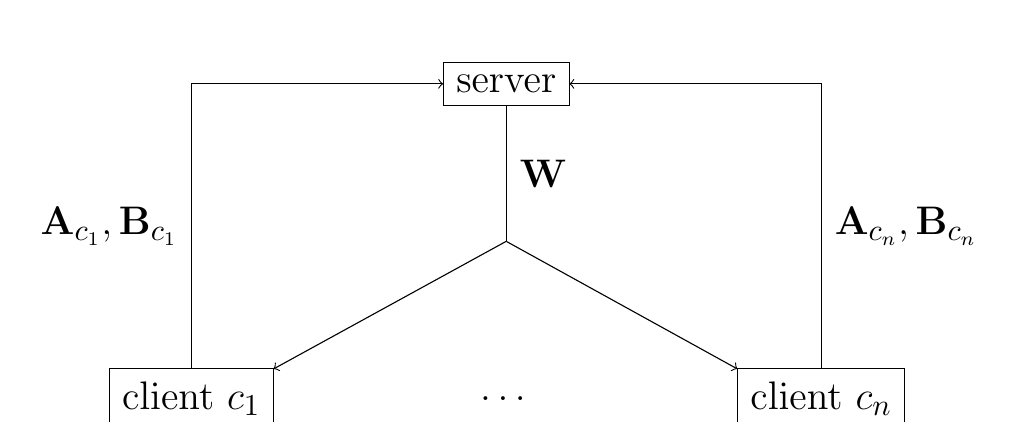
\begin{tikzpicture}[scale=2]
  \draw[line width=0pt]
    (2,2) node[draw] (s) {server}
    (0,0)  node[draw] (c1) {client $c_1$}
    (4,0)  node[draw] (cn) {client $c_n$}
    (2,0)  node[draw=none] (d) {$\dots$};

  \draw[->] (2,1)--(c1.north east);
  \draw[->] (2,1)--(cn.north west);
  \draw (2,1)-- node[right] {$\textbf{W}$} (s);
  \draw[->] (c1.north)-- node[left] {$\textbf{A}_{c_1},\textbf{B}_{c_1}$} (0,2)--(s.west);
  \draw[->] (cn.north)-- node[right] {$\textbf{A}_{c_n},\textbf{B}_{c_n}$} (4,2)--(s.east);
\end{tikzpicture}
\caption{Incremental Federated Learning Scheme. Each client sends their local matrices $\textbf{A}_c$ and $\textbf{B}_c$ to the server. After the matrices are aggregated and multiplied to compute the optimal readout weights, the server transmits $\textbf{W}$ back to all clients \cite{bacciu2021federated}.}
\end{figure}


This method shows how the use of ESNs, which are efficient state-of-the-art RNN models for time-series processing, enables a form of federation that is optimal in the sense that it produces models mathematically equivalent to the corresponding centralized model. This is the baseline, or a starting point, for the FL part of this Work that tries to achieve, or even surpass, the state-of-the-art results.

\chapter{Federated Curvature for Echo State Networks}\label{chapter:fedcurv}

In this Chapter are described the federated settings and the implementation details of the Federated Curvature (\texttt{FedCurv}) algorithm applied to the ESN, following the theoretical aspects explained in Section \ref{sec:fedcurv}. \\

The Federated Learning scenario of the ESNs starts initializing the server ESN model parameters $\textbf{W}_{in}\in \mathbb{R}^{N_x\times N_u}$, $\widehat{\textbf{W}}\in \mathbb{R}^{N_x\times N_x}$, $\textbf{W}\in \mathbb{R}^{N_y\times N_x}$, $u_{server}\in \mathbb{R}^{N_y\times N_x}$ and $v_{server}\in \mathbb{R}^{N_y\times N_x}$; $N_x$ is the number of reservoir neurons, $N_u$ is the input dimension, $N_y$ is the output dimension, $u_{server}$ and $v_{server}$ are, respectively, the importance of the \textbf{W} parameters for the task at time $t$ and the importance of the same parameters at time $t-1$. We focus our attention on \textbf{W} because they are the only parameters trained in the learning process. \\

The clients ESN models have the same structure of the server, the clients models parameters could be initialized as the same of the server parameters or differently from the server. \\

After the initialization of the federated nodes, the server broadcasts to the clients the \textbf{W}, $u_{server}$ and $v_{server}$ parameters; $u_{server}$ and $v_{server}$ are initialized as zero tensors at the beginning. For each batch of local data and for each round, each client computes predictions ($\textbf{y}(t)$) on that data. The outputs are used to penalize the local client parameters that goes too far from the previous task, and so from \textbf{W} received from the server. To do so, we compute the gradient of the log-likelihood of the predictions with respect to the \textbf{W} parameters. The gradient is computed as $\frac{\partial log(softmax(\textbf{y}(t)))}{\partial w}$ and it is squared and normalized by the length of the batch of data in order to get our approximation of the diagonal of the Fisher matrix; This tells us the importance of each parameter. \\

After computing the Fisher diagonal ($\mathcal{D}$), we need to penalize the client for going "far from the server". To do so each client considers $u=\mathcal{D}$ and $v=\mathcal{D}\times \textbf{W}$, but in order to penalize with respect to the importance of the other clients, we need to subtract $u$ and $v$, respectively, from $u_{server}$ and $v_{server}$; so $u_{client}=u_{server}-u$ and $v_{client}=v_{server}-v$. The penalty term is computed as $\lambda= sum(\textbf{W}^2\times u_{local}-2\times \textbf{W}\times v_{local})$ (as shown in Eq. \ref{eq:fedcurv_obj}) and added to the loss function to perform the optimization step and compute the $\textbf{W}_{client}$ parameters.  \\

After updating the client parameters, each client broadcast to the server it's own  $\textbf{W}_{client}$, $u_{client}$ and $v_{client}$. The server assign to \textbf{W} the average of the $\textbf{W}_{client}$ received from the clients and it updates $u_{server}$ and $v_{server}$, respectively, summing the $u_{client}$ and $v_{client}$ received from the clients. \\

The pseudo-code of the \texttt{FedCurv} algorithm is shown in Alg. \ref{alg:fedcurv}. \\


\algrenewcommand\algorithmicfunction{}
\algrenewcommand\textproc{}
\begin{algorithm}[H]
\caption{\texttt{FedCurv}. The $K$ clients are indexed by $k$; $B$ is the local minibatch size, $E$ is the number of local epochs, and $\eta$ is the learning rate. Each client has the reservoir parameter $\textbf{W}_{in}$ and $\widehat{\textbf{W}}$, $\alpha$ is the leaky rate, $N_y$ is the output dimension and $N_x$ is the number of reservoir neurons.}\label{alg:fedcurv}
\begin{algorithmic}[1]
\Function{\textbf{ServerUpdate}}{}
    \State let $w_0, u_0, v_0\in \mathbb{R}^{N_y\times N_x}$
    \For{\texttt{each round $t=1,2,\dots$}}
        \State $m\leftarrow \max(C\cdot K, 1)$
        \State $S_t\leftarrow \text{(random set of $m$ clients)}$
        \For{\texttt{each client $k\in S_t$}}
            \State $w_{t+1}^k, u_{t+1}^k, v_{t+1}^k\leftarrow$ \text{ClientUpdate($k$, $w_t$, $u_t$, $v_t$)}
        \EndFor
        \State $w_{t+1}\leftarrow \sum_{k=1}^K\frac{n_k}{n}w_{t+1}^k$
        \State $u_{t+1}\leftarrow \sum_{k=1}^K u_{t+1}^k$
        \State $v_{t+1}\leftarrow \sum_{k=1}^K v_{t+1}^k$
    \EndFor
\EndFunction
\\
\Function{\textbf{ClientUpdate}}{$k$, $w$, $u$, $v$}
    \State let $u_{local}, v_{local}\in \mathbb{R}^{N_y\times N_x}$
    \State $\mathcal{B}\leftarrow \text{(split $\mathcal{P}_k$ into batches of size $B$)}$
    \For{\texttt{$i$ from $1$ to $E$}}
        \For{\text{batch $b\in \mathcal{B}$}}
            \State $\textbf{x}(t)=(1-\alpha)\textbf{x}(t-1)+\alpha \tanh(\textbf{W}_{in}b+\widehat{\textbf{W}}\textbf{x}(t-1))$
            \State $\textbf{y}(t)\leftarrow sigmoid(w\textbf{x}(t))$
            \State $\nabla\mathcal{LL}_b\leftarrow\frac{\partial log(softmax(\textbf{y}(t)))}{\partial w}$ \Comment{Log-likelihood gradient}
            \State $\mathcal{D}_b\leftarrow\frac{(\nabla\mathcal{LL}_b)^{2}}{length(b)}$ \Comment{Diagonal of the Fisher matrix}
            \State $u_b\leftarrow\mathcal{D}_b$
            \State $v_b\leftarrow\mathcal{D}_b\times w$
            \State $u_{local} \leftarrow u-u_b$
            \State $v_{local} \leftarrow v-v_b$
            \State $\lambda\leftarrow sum(w^2\times u_{local}-2\times w\times v_{local})$ \Comment{Penalty term}
            \State $w\leftarrow w-\eta\nabla[\ell(w;b)+\lambda]$
        \EndFor
    \EndFor
    \Return $w, u_{local}, v_{local}$
\EndFunction
\end{algorithmic}
\end{algorithm}

The diagram of the federated process with the elements exchanged by clients and server is shown in Fig. \ref{fig:fedcurv}.

\begin{figure}[H]
\centering
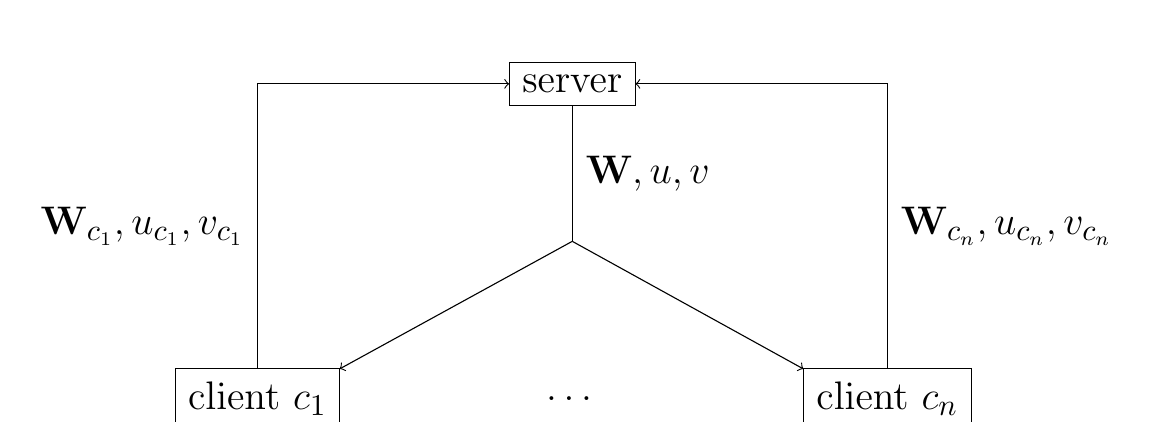
\begin{tikzpicture}[scale=2]
  \draw[line width=0pt]
    (2,2) node[draw] (s) {server}
    (0,0)  node[draw] (c1) {client $c_1$}
    (4,0)  node[draw] (cn) {client $c_n$}
    (2,0)  node[draw=none] (d) {$\dots$};

  \draw[->] (2,1)--(c1.north east);
  \draw[->] (2,1)--(cn.north west);
  \draw (2,1)-- node[right] {$\textbf{W},u,v$} (s);
  \draw[->] (c1.north)-- node[left] {$\textbf{W}_{c_1},u_{c_1},v_{c_1}$} (0,2)--(s.west);
  \draw[->] (cn.north)-- node[right] {$\textbf{W}_{c_n},u_{c_n},v_{c_n}$} (4,2)--(s.east);
\end{tikzpicture}
\caption{Federated Curvature Scheme. Each client $c$ sends their local matrix $\textbf{W}_c$, $u_c$ and $v_c$ to the server. After the aggregation of the models is performed in the form of a weighted average of the $\textbf{W}_c$, the sum of the $u_c$ and the sum of the $v_c$, the server sends back the same parameters $\textbf{W}$, $u$ and $v$ to all clients.\\}
\label{fig:fedcurv}
\end{figure}


The implementation has be done using Tensorflow-Federated (TFF) framework\footnote{\url{https://www.tensorflow.org/federated}} due to the natural compatibility with Tensorflow (TF) framework\footnote{\url{https://www.tensorflow.org/}} that it is used for the models implementations. TFF is an open-source framework for machine learning and other computations on decentralized data and has been developed to facilitate open research and experimentation with FL. A research FL simulation implemented in TFF typically consists of three main types of logic:

\begin{enumerate}
    \item Individual pieces of TF  code, typically \hltexttt{tf.function}\footnote{\url{https://www.tensorflow.org/api_docs/python/tf/function}}, that encapsulate logic that runs in a single location (e.g., on clients or on a server). This code is typically written and tested without any \hltexttt{tff.*} references, and can be re-used outside of TFF
    
    \item TFF orchestration logic, which binds together the individual \hltexttt{tf.function} from 1) by wrapping them as \hltexttt{tff.tf\_computation}\footnote{\url{https://www.tensorflow.org/federated/api_docs/python/tff/tf_computation}} and then orchestrating them using abstractions like \hltexttt{tff.federated\_broadcast}\footnote{\url{https://www.tensorflow.org/federated/api_docs/python/tff/federated_broadcast}} and \hltexttt{tff.federated\_mean}\footnote{\url{https://www.tensorflow.org/federated/api_docs/python/tff/federated_mean}} inside a \hltexttt{tff.federated\_computation}
    
    \item An outer driver script that simulates the control logic of a production FL system, selecting simulated clients from a dataset and then executing federated computations defined in 2).
\end{enumerate}


For the basic \texttt{FedAvg} algorithm we use the \\ \hltexttt{tff.learning.build\_federated\_averaging\_process} built-in function. It uses the \hltexttt{model\_fn} function to initialize the server and clients models, the \hltexttt{client\_optimizer\_fn} to update the clients and \hltexttt{server\_optimizer\_fn} to update the server. Then, an initial state is instantiated and updated at each round. The \texttt{FedAvg} iterative process is shown in Listing \ref{code:fedavg_iter_proc}. \\


\begin{lstlisting}[caption={Example code of the TFF iterative process for \texttt{FedAvg}.},label={code:fedavg_iter_proc},language=Python]
import tensorflow as tf
import tensorflow_federated as tff

fedavg_iter_process = tff.learning.build_federated_averaging_process(
        model_fn,
        client_optimizer_fn,
        server_optimizer_fn)
        
state = fedavg_iter_process.initialize()

for round in range(NUM_ROUNDS):
    state = fedavg_iter_process.next(state, training_dataset)
\end{lstlisting}


Concerning the \texttt{FedCurv} algorithm, there isn't a build-in function in TFF, so the iterative process has been done from scratch, that is shown in Listing \ref{code:fedcurv_iter_proc}.


\begin{lstlisting}[caption={Example code of the TFF iterative process for \texttt{FedCurv}.},label={code:fedcurv_iter_proc},language=Python]
import tensorflow as tf
import tensorflow_federated as tff

fedcurv_iter_process = tff.templates.IterativeProcess(
      initialize_fn=server_init_tff,
      next_fn=next_fn)
      
state = fedcurv_iter_process.initialize()

for round in range(NUM_ROUNDS):
    state = fedcurv_iter_process.next(state, training_dataset)
\end{lstlisting}


In the \hltexttt{next\_fn} function are executed the \hltexttt{ServerUpdate} and \hltexttt{ClientUpdate} functions of the Alg. \ref{alg:fedcurv}. In Listing \ref{code:fedcurv_next_fn} there is the implementation of the \hltexttt{next\_fn} that is the central point of the parameters dispatching from server to clients and vice versa. In the \hltexttt{next\_fn} the server parameters are broadcasted to each clients and used to update the clients by using the \hltexttt{client\_update\_fn} function; then the clients parameters are collected and aggregated and send to the server for updating by the use of \hltexttt{server\_update\_fn}. \\


\begin{lstlisting}[caption={TFF implementation of the next\_fn of \texttt{FedCurv}.},label={code:fedcurv_next_fn},language=Python]
@tff.federated_computation(federated_server_type, federated_dataset_type)
  def next_fn(server_state, federated_dataset):
    # Broadcast the server weights to the clients.
    server_state_at_client = tff.federated_broadcast(server_state)
    server_weights_at_client = server_state_at_client.trainable_weights
    u_global_at_client = server_state_at_client.u_global
    v_global_at_client = server_state_at_client.v_global
    # Local client update.
    model_deltas, u_locals, v_locals = tff.federated_map(
        client_update_fn, 
        (federated_dataset, server_weights_at_client, u_global_at_client, v_global_at_client))
    # Client-to-server upload and aggregation.
    mean_model_delta = tff.federated_mean(model_deltas)
    u_sum = tff.federated_sum(u_locals)
    v_sum = tff.federated_sum(v_locals)
    # Server update.
    server_state = tff.federated_map(
        server_update_fn, (server_state, mean_model_delta, u_sum, v_sum))
    return server_state
\end{lstlisting}

The \hltexttt{client\_update\_fn} and \hltexttt{server\_update\_fn} are shown, respectively, in Listing \ref{code:client_update_fn} and \ref{code:server_update_fn}. \\


\begin{lstlisting}[caption={TFF implementation of the client\_update\_fn of \texttt{FedCurv}.},label={code:client_update_fn},language=Python]
@tf.function
  def client_update(model, dataset, server_weights, server_u, server_v):
    fish_tmp = [tf.zeros_like(tensor) for tensor in model.trainable_variables]
    u_local = [tf.zeros_like(tensor) for tensor in server_u]
    v_local = [tf.zeros_like(tf.multiply(f, w)) for f,w in zip(fish_tmp, server_v)]
    client_weights_old = [tf.zeros_like(tensor) for tensor in model.trainable_variables]
    client_weights_new = [tf.zeros_like(tensor) for tensor in model.trainable_variables]
    updated_weights = [tf.zeros_like(tensor) for tensor in model.trainable_variables]
    
    client_weights_old = model.trainable_variables
    client_weights_new = model.trainable_variables
    updated_weights = model.trainable_variables
    
    for batch in iter(dataset):
      fish_diag = fisher_matrix(model, batch)
      u_local = [fim for fim in fish_diag]
      v_local = [tf.multiply(fim, w_old) for fim, w_old in zip(fish_diag, client_weights_old)]
      penalty = compute_penalty(batch, client_weights_new, server_u, server_v, u_local, v_local)
      
      with tf.GradientTape() as tape:
        outputs = model.forward_pass(batch)
        loss = outputs.loss + penalty
        grads = tape.gradient(loss, model.trainable_variables)
        optimizer_state, updated_weights = client_optimizer.next(optimizer_state, client_weights_new, grads)
      
      client_weights_old = client_weights_new
      client_weights_new = updated_weights
    return tf.nest.map_structure(tf.subtract, client_weights_new, server_weights), u_local, v_local
\end{lstlisting}

\begin{lstlisting}[caption={TFF implementation of the server\_update\_fn of \texttt{FedCurv}.},label={code:server_update_fn},language=Python]
@tf.function
  def server_update(server_state, mean_model_delta, u_sum, v_sum):
    negative_weights_delta = tf.nest.map_structure(lambda w: -1.0 * w, mean_model_delta)
    new_optimizer_state, updated_weights = server_optimizer.next(
        server_state.optimizer_state, server_state.trainable_weights, 
        negative_weights_delta)
    
    return tff.structure.update_struct(
        server_state,
        model=tff.learning.ModelWeights(
            trainable=updated_weights,
            non_trainable=server_state.model.non_trainable
        ),
        trainable_weights=updated_weights,
        optimizer_state=new_optimizer_state,
        u_global=u_sum,
        v_global=v_sum)
\end{lstlisting}


The two essential components of \texttt{FedCurv} are the computation of the diagonal of the Fisher Information matrix and the computation of the penalty term. Concerning the computation of the Fisher Information matrix, this is shown in Listing \ref{code:fim}.


\begin{lstlisting}[caption={Code for the computation of the diagonal of the Fisher Information matrix.},label={code:fim},language=Python]
import tensorflow as tf
import tensorflow_federated as tff

def fisher_diag(model, batch):
  weights = model.trainable_variables
  n_samples = len(batch)
  fisher_diagonal = [tf.zeros_like(tensor) for tensor in weights]
  with tf.GradientTape() as tape:
    output = model.forward_pass(batch).predictions
    log_likelihood = tf.nn.log_softmax(output)
    gradients = tape.gradient(log_likelihood, weights)
  fisher_diagonal = [(grad**2)/n_samples for grad in gradients]
  return fisher_diagonal
\end{lstlisting}


Instead, the computation of the penalty term is shown in Listing \ref{code:penalty}.


\begin{lstlisting}[caption={Code for the computation of the penalty term.},label={code:penalty},language=Python]
import tensorflow as tf
import tensorflow_federated as tff

def compute_penalty(weights, u_global, v_global, u_local, v_local):
  penalty = 0.
  for w, u_g, v_g, u_l, v_l in zip(weights, u_global, v_global, u_local, v_local):
      u = u_g - u_l
      v = v_g - v_l
      penalty += tf.reduce_sum((w**2)*u - 2*w*v)
  return 1e-4*penalty
\end{lstlisting}

\chapter{Discriminator for Anomalous Client detection}\label{chapter:disc}

A common need when analyzing real-world data-sets is determining which instances stand out as being dissimilar to all others. Such instances are known as \textit{anomalies}, and the goal of \textit{anomaly detection} (also known as outlier detection) is to determine all such instances in a data-driven fashion \cite{chandola2007outlier}. Anomalies can be caused by errors in the data but sometimes are indicative of a new, previously unknown, underlying process. In the broader field of machine learning, the recent years have witnessed a proliferation of deep neural networks, with unprecedented results across various application domains. Deep learning (DL) is a subset of ML that achieves good performance and flexibility by learning to represent the data as a nested hierarchy of concepts within layers of the neural network. \\

Anomalies are also referred to as abnormalities, deviants, or outliers in the data mining and statistics literature \cite{aggarwal2017introduction}. Despite the substantial advances made by DL methods in many ML problems, there is a relative scarcity of DL approaches for anomaly detection \cite{chalapathy2019deep}. \\

Anomalies can be broadly classified into three types: \textit{point anomalies}, \textit{contextual anomalies} and \textit{collective anomalies}.

\begin{enumerate}
    \item \textit{Point anomaly}: represents a point which stands on a low-density region of the observed distribution;
    
    \item \textit{Contextual anomaly}: represents an observation which is not a point anomaly but it is anomalous with respect to the surrounding context in the sequence of observations;
    
    \item \textit{Collective anomalies}: are anomalies that arise from the observations of the distributions across multiple data streams.
\end{enumerate}

The type of anomaly considered in this Work refers to \textit{point anomalies}. Specifically, we want to detect anomalous client at a certain time. This detection has to be done server side, due to privacy concerns and low computational power at edge devices. \\

There are a lot of anomaly detection topics like: intrusion detection, fraud detection, banking fraud, malware detection, IoT Big Data anomaly detection, industrial anomalies detection, etc \cite{chalapathy2019deep}. Among them, we can't find something related to "anomalous machine learning model" detection. \\

In this chapter is described the approach used to identify anomalous clients during the FL process. The scope is to detect/discriminate and discard those clients, in order to not considering them during the process of an FL algorithm. In this way the aggregated model will not be affected by anomalous clients. \\

Our approach is to train a simple feedforward neural network on the gradients of clients computed at each backpropagation step, in order to distinguish between: client trained on noisy input and client trained on plain input. The reason of using the clients' gradients comes from the fact that those are the only things that clients share with the server. The gradient taken into account is computed making a subtraction between the weights at time $t$ and at time $t-1$. Concerning the implementation with Tensorflow-Federated, the discriminator is added into the \hltexttt{client\_update\_fn} and following the same structure and components described in Chapter \ref{chapter:fedcurv}. \\

The discriminator model is made with the Tensorflow\footnote{\url{https://www.tensorflow.org/}} framework with two \hltexttt{Dense}\footnote{\url{https://www.tensorflow.org/api_docs/python/tf/keras/layers/Dense}} layers, two \hltexttt{Dropout}\footnote{\url{https://www.tensorflow.org/api_docs/python/tf/keras/layers/Dropout}} layer (one after each \hltexttt{Dense} layer) and a \hltexttt{Dense} output layer with \hltexttt{Sigmoid} activation function. \\

The \texttt{FedAvg} and \texttt{FedCurv} algorithms with the discriminator (\texttt{Disc}) are described, respectively, in the Alg. \ref{alg:fedavg+disc} and \ref{alg:fedcurv+disc}.


\algrenewcommand\algorithmicfunction{}
\algrenewcommand\textproc{}
\begin{algorithm}[H]
\caption{\texttt{FedAvg+Disc}. The $K$ clients are indexed by $k$; $B$ is the local minibatch size, $E$ is the number of local epochs, and $\eta$ is the learning rate.}\label{alg:fedavg+disc}
\begin{algorithmic}[1]
\Function{\textbf{ServerUpdate}}{}
    \State $w_0\leftarrow$ initialize()
    \State $disc\leftarrow \text{(load $\texttt{Disc}$ model)}$
    \For{\texttt{each round $t=1,2,\dots$}}
        \State $m\leftarrow \max(C\cdot K, 1)$
        \State $S_t\leftarrow \text{(random set of $m$ clients)}$
        \For{\texttt{each client $k\in S_t$}}
            \State $w_{t+1}^k\leftarrow$ \text{ClientUpdate($k$, $w_t$)}
            \State $valid\leftarrow disc(w_t^k-w_{t+1}^k)$
            \If{not $valid$}
                $w_{t+1}^k\leftarrow w_t^k$
            \EndIf
        \EndFor
        \State $w_{t+1}\leftarrow \sum_{k=1}^K\frac{n_k}{n}w_{t+1}^k$
    \EndFor
\EndFunction
\\
\Function{\textbf{ClientUpdate}}{$k$, $w$}
    \State $\mathcal{B}\leftarrow \text{(split $\mathcal{P}_k$ into batches of size $B$)}$
    \For{\texttt{$i$ from $1$ to $E$}}
        \For{\text{batch $b\in \mathcal{B}$}}
            \State $w\leftarrow w-\eta\nabla\ell(w;b)$
        \EndFor
    \EndFor
    \Return $w$
\EndFunction
\end{algorithmic}
\end{algorithm}


\algrenewcommand\algorithmicfunction{}
\algrenewcommand\textproc{}
\begin{algorithm}[H]
\caption{\texttt{FedCurv+Disc}. The $K$ clients are indexed by $k$; $B$ is the local minibatch size, $E$ is the number of local epochs, and $\eta$ is the learning rate. Each client has the reservoir parameter $\textbf{W}_{in}$ and $\widehat{\textbf{W}}$, $\alpha$ is the leaky rate, $N_y$ is the output dimension and $N_x$ is the number of reservoir neurons.}\label{alg:fedcurv+disc}
\begin{algorithmic}[1]
\Function{\textbf{ServerUpdate}}{}
    \State let $w_0, u_0, v_0\in \mathbb{R}^{N_y\times N_x}$
    \For{\texttt{each round $t=1,2,\dots$}}
        \State $m\leftarrow \max(C\cdot K, 1)$
        \State $S_t\leftarrow \text{(random set of $m$ clients)}$
        \For{\texttt{each client $k\in S_t$}}
            \State $w_{t+1}^k, u_{t+1}^k, v_{t+1}^k\leftarrow$ \text{ClientUpdate($k$, $w_t$, $u_t$, $v_t$)}
            \State $valid\leftarrow disc(w_t^k-w_{t+1}^k)$
            \If{not $valid$}
                $w_{t+1}^k\leftarrow w_t^k$
            \EndIf
        \EndFor
        \State $w_{t+1}\leftarrow \sum_{k=1}^K\frac{n_k}{n}w_{t+1}^k$
        \State $u_{t+1}\leftarrow \sum_{k=1}^K u_{t+1}^k$
        \State $v_{t+1}\leftarrow \sum_{k=1}^K v_{t+1}^k$
    \EndFor
\EndFunction
\\
\Function{\textbf{ClientUpdate}}{$k$, $w$, $u$, $v$}
    \State let $u_{local}, v_{local}\in \mathbb{R}^{N_y\times N_x}$
    \State $\mathcal{B}\leftarrow \text{(split $\mathcal{P}_k$ into batches of size $B$)}$
    \For{\texttt{$i$ from $1$ to $E$}}
        \For{\text{batch $b\in \mathcal{B}$}}
            \State $\textbf{x}(t)=(1-\alpha)\textbf{x}(t-1)+\alpha \tanh(\textbf{W}_{in}b+\widehat{\textbf{W}}\textbf{x}(t-1))$
            \State $\textbf{y}(t)\leftarrow sigmoid(w\textbf{x}(t))$
            \State $\nabla\mathcal{LL}_b\leftarrow\frac{\partial log(softmax(\textbf{y}(t)))}{\partial w}$ \Comment{Log-likelihood gradient}
            \State $\mathcal{D}_b\leftarrow\frac{(\nabla\mathcal{LL}_b)^{2}}{length(b)}$ \Comment{Diagonal of the Fisher matrix}
            \State $u_b\leftarrow\mathcal{D}_b$
            \State $v_b\leftarrow\mathcal{D}_b\times w$
            \State $u_{local} \leftarrow u-u_b$
            \State $v_{local} \leftarrow v-v_b$
            \State $\lambda\leftarrow sum(w^2\times u_{local}-2\times w\times v_{local})$ \Comment{Penalty term}
            \State $w\leftarrow w-\eta\nabla[\ell(w;b)+\lambda]$
        \EndFor
    \EndFor
    \Return $w, u_{local}, v_{local}$
\EndFunction
\end{algorithmic}
\end{algorithm}

\chapter{Data Preparation}\label{chapter:dataset}

In this Chapter are described the WESAD Dataset \cite{schmidt2018introducing} for stress prediction in Section \ref{sec:wesad}, and the pre-processing phase in Section \ref{sec:data_preproc} in order to  increasing the ESNs stress prediction performances.


\section{WESAD Dataset}\label{sec:wesad}

Affect recognition aims to detect a person’s affective state based on observables, with the goal to improve human-computer interaction. WESAD is a publicly available dataset for wearable stress and affect detection. This multimodal dataset features physiological and motion data, recorded from both a wrist/chest-worn device, of 15 subjects during a lab study. For our purposes, we consider the chest device data, and specifically the Electrodermal Activity (EDA), sampled at 4HZ, and the Blood Volume Pulse (BVP), sampled at 64 Hz. The signals are associated to specific label:

\begin{itemize}
    \item Baseline
    \item Stress
    \item Amusement
    \item Meditation
\end{itemize}

We want to solve the binary classification problem of predicting if a user is stressed or not. So, the signals associated to labels different from \textit{Stress}, are considered as "Not Stressed" (associated to the integer value 0), the other signals associated to the label \textit{Stress}, obviously, are considered as "Stressed" (associated to the integer value 1).


\section{Data Preprocessing}\label{sec:data_preproc}

The Data pre-processing phase starts from EDA and BVP signals of the 15 subjects. In the initial phase it is used the NeuroKit2 library\footnote{\url{https://github.com/neuropsychology/NeuroKit}}, a Python Toolbox for Neurophysiological Signal Processing. The EDA signals are cleaned using the function \hltexttt{eda\_clean}\footnote{\url{https://neuropsychology.github.io/NeuroKit/functions/eda.html#neurokit2.eda.eda_clean}}. The BVP signal, instead, could be considered similar to Photoplethysmogram (PPG) signal (used to detect blood volume changes in the microvascular bed of tissue), and for this reason it is cleaned using the function \hltexttt{ppg\_clean}\footnote{\url{https://neuropsychology.github.io/NeuroKit/functions/ppg.html#neurokit2.ppg.ppg_clean}}. \\

In the second phase, from the EDA signals are extracted another two features: EDA Thonic (tEDA) and EDA Phasic (pEDA); this is done using the function \hltexttt{eda\_phasic}\footnote{\url{https://neuropsychology.github.io/NeuroKit/functions/eda.html#neurokit2.eda.eda_phasic}}. Consequently, the BVP signals are used to find the PPG peaks by using the function \hltexttt{ppg\_findpeaks}\footnote{\url{https://neuropsychology.github.io/NeuroKit/functions/ppg.html#neurokit2.ppg.ppg_findpeaks}}. The peaks are used to extract the Heart Rate (HR), using the function \hltexttt{ppg\_rate}\footnote{\url{https://neuropsychology.github.io/NeuroKit/functions/signal.html#signal-rate}}. The peaks are used also to compute the Heart Rate Variability (HRV), that is done using the function \hltexttt{hrv\_time}\footnote{\url{https://neuropsychology.github.io/NeuroKit/functions/hrv.html#neurokit2.hrv.hrv_time}} applied to a sliding window on the PPG peaks signal. The sliding windows considered are of the length of: 5, 25 and 50, and it is multiplied by 64 (the sampling frequency of BVP/PPG) in order to consider a timing of seconds. \\

The result of the previous phases, results in a definition of 3 different dataset (one for each sliding window) with the following fields for each subject:

\begin{enumerate}
    \item tEDA: EDA Thonic
    \item pEDA: EDA Phasic
    \item HR: Heart Rate
    \item HRV: Heart Rate Variability (sliding window $\in \{5, 25, 50\}$)
    \item Label: Stressed or Not Stressed (1 or 0).
\end{enumerate}

The statistics of the dataset after the second phase are shown in Table \ref{tab:data_1}.

{\renewcommand{\arraystretch}{1.5}
\begin{table}[H]
    \centering
    \begin{tabular}{|c|c|c|c|c|}
        \hline
        Feature & Min & Max & Mean & Var \\ \hline\hline
        pEDA & -4.4867 & 5.8884 & -0.0140 & 0.9325 \\ \hline
        tEDA & 0.1639 & 9.6628 & 1.8536 & 4.3981 \\ \hline
        HR & 0.4868 & 192.0000 & 77.7142 & 770.1333 \\ \hline
        HRV & 12.9829 & 386.3441 & 45.8408 & 3245.0130 \\ \hline
    \end{tabular}
    \caption{Dataset statistics of the extracted features with a sliding window of $25\times 64$. Percentage of samples: label "0": 88.53\%, label "1": 11.47\%}
    \label{tab:data_1}
\end{table}

The third phase consists in resampling the signals with respect to the shortest one for each subject, this is done using the function \hltexttt{signal\_resample}\footnote{\url{https://neuropsychology.github.io/NeuroKit/functions/signal.html#neurokit2.signal_resample}}. Next, the signals of each subject are standardized with respect to its own baseline, in order to recenter the signals in an interval more appropriate for the ESN, this is done using the \hltexttt{StandardScaler}\footnote{\url{https://scikit-learn.org/stable/modules/generated/sklearn.preprocessing.StandardScaler.html}} of the \hltexttt{sklearn}\footnote{\url{https://scikit-learn.org}} library.

The statistics of the standardized dataset after the third phase are shown in Table \ref{tab:data_2}.

{\renewcommand{\arraystretch}{1.5}
\begin{table}[H]
    \centering
    \begin{tabular}{|c|c|c|c|c|}
        \hline
        Feature & Min & Max & Mean & Var \\ \hline\hline
        pEDA & -46.4578 & 134.4446 & 0.9768 & 133.8697 \\ \hline
        tEDA & -11.2772 & 67.8104 & 4.6638 & 139.6957 \\ \hline
        HR & -4.9910 & 7.4297 & 0.1300 & 1.6040 \\ \hline
        HRV & -3.3037 & 92.1442 & 3.9575 & 108.4837 \\ \hline
    \end{tabular}
    \caption{Dataset statistics of the standardized features with a sliding window of $25\times 64$. Percentage of samples: label "0": 88.57\%, label "1": 11.43\%}
    \label{tab:data_2}
\end{table}

The last phase is a normalization of the features with an online moving average. The statistics of the normalized dataset are shown in Table \ref{tab:data_3}.


{\renewcommand{\arraystretch}{1.5}
\begin{table}[H]
    \centering
    \begin{tabular}{|c|c|c|c|c|}
        \hline
        Feature & Min & Max & Mean & Var \\ \hline\hline
        pEDA & -2.9826 & 6.8522 & 0.6837 & 2.4992 \\ \hline
        tEDA & -20053.9745 & 12748.3417 & 0.6757 & 8039.7497 \\ \hline
        HR & -278.8295 & 537.7899 & 1.1065 & 264.5812 \\ \hline
        HRV & -4.5778 & 21.5005 & 1.1469 & 7.9482 \\ \hline
    \end{tabular}
    \caption{Dataset statistics of the normalized features with moving average with a sliding window of $25\times 64$. Percentage of samples: label "0": 88.57\%, label "1": 11.43\%}
    \label{tab:data_3}
\end{table}

The last dataset contains $\sim 6000$ samples for each subject and it is the one used for the Experimental phase in Chapter \ref{chapter:experiments}.

\chapter{Experiments}\label{chapter:experiments}

In this Chapter we are going to describe the hyper-parameter search and the final structure of the best ESN on the stress prediction task. Next, we will show the settings of the ESN model, found in the previous phase, applied to the FL scenario; these phases are described in Section \ref{sec:setup}. In Section \ref{sec:results} are shown the results concerning the FL scenarios (Alg. \ref{alg:fedavg} and \ref{alg:fedcurv}) and the FL scenarios with the use of a discriminator for anomalous client detection (Alg. \ref{alg:fedavg+disc} and \ref{alg:fedcurv+disc}).


\section{Experimental Setup}\label{sec:setup}

The experiments are conducted using the Python programming language and the Machine Learning models are written using the Tensorflow framework with the Keras backend. The \textit{reservoir} of the ESN has been implemented using the Tensorflow Addons\footnote{\url{https://www.tensorflow.org/addons}} library, and specifically the \hltexttt{ESN}\footnote{\url{https://www.tensorflow.org/addons/api_docs/python/tfa/layers/ESN}} layer. The \textit{readout} of the ESN has been implemented using a simple \hltexttt{Dense}\footnote{\url{https://www.tensorflow.org/api_docs/python/tf/keras/layers/Dense}} layer with \hltexttt{Sigmoid}\footnote{\url{https://www.tensorflow.org/api_docs/python/tf/keras/activations/sigmoid}} activation function and \hltexttt{class\_weight=\{0: 12, 1: 88\}} in order to takle the problem of unbalanced labels distribution (see Table \ref{tab:data_3}). The model is compiled using the \hltexttt{Adam} optimizer\footnote{\url{https://www.tensorflow.org/api_docs/python/tf/keras/optimizers/Adam}} and \hltexttt{BinaryCrossentropy}\footnote{\url{https://www.tensorflow.org/api_docs/python/tf/keras/losses/BinaryCrossentropy}} loss function. \\

The \textit{model selection} phase is conducted using the KerasTuner\footnote{\url{https://keras.io/keras_tuner/}} library. Specifically, it is used the \hltexttt{RandomSearch}\footnote{\url{https://keras.io/api/keras_tuner/tuners/random/}} class that uses a set of \hltexttt{HyperParameters}\footnote{\url{https://keras.io/api/keras_tuner/hyperparameters/}} values to explore the search space in a random way. The dataset has been splitted in \textit{training set} containing 10 subjects, \textit{validation set} containing 4 subjects and \textit{test set} with just one subject. The search is interrupted when all the hypothesis has been exhausted. The hyper-parameter search space is shown in Table \ref{tab:grid_search}.


{\renewcommand{\arraystretch}{1.5}
\begin{table}[H]
    \centering
    \begin{tabular}{|l||c|}
        \hline
        Units & $50, 100, 200$ \\ \hline
        Leaky ($\alpha$) & $0.5, 0.8, 1.0$ \\ \hline
        Learning rate ($\eta$) & $0.001, 0.01, 0.1$ \\ \hline
        Window size & $(5\times 64), (25\times 64), (50\times 64)$ \\ \hline
        Batch size & $20, 50, 100$ \\ \hline
        Features & (pEDA, tEDA, HR, HRV), \\
        & (tEDA, pEDA), (HR, HRV), \\
        & (pEDA) \\ \hline
    \end{tabular}
    \caption{ESN hyper-parameter search space.}
    \label{tab:grid_search}
\end{table}


The best model parameters has been chosen looking at the F1 score (the harmonic mean of the precision and recall) on the \textit{validation set}. The reason why using the F1 score is that it is more suitable for task with unbalanced class distribution. In Table \ref{tab:best_model} are shown the best parameters associated with a validation F1 score of \texttt{0.9106}.

{\renewcommand{\arraystretch}{1.5}
\begin{table}[H]
    \centering
    \begin{tabular}{|c|c|c|c|c|c|c|c|}
        \hline
        Units & $\alpha$ & $\eta$ & $\rho$ & Window & Batch & Features & Epochs \\ \hline\hline
        200 & 1.0 & 0.1 & 0.99 & $25\times 64$ & 20 & pEDA & 1 \\ \hline
    \end{tabular}
    \caption{Best ESN model parameters associated with a validation F1 score of \texttt{0.9106}.}
    \label{tab:best_model}
\end{table}

A graphical representation of the  architecture of the model is shown in Fig \ref{fig:esn}.

\begin{center}
\begin{minipage}[c]{\textwidth}
    \centering
    \includegraphics[width=0.7\textwidth]{contents/Chapter6/esn.png}
    \captionof{figure}{ESN model architecture.}
    \label{fig:esn}
\end{minipage}
\end{center}

In the \textit{model assessment} phase, the ESN has been re-trained on the entire \textit{design set} and having the final performances shown in Table \ref{tab:best_model_perf}.

{\renewcommand{\arraystretch}{1.5}
\begin{table}[H]
    \centering
    \begin{tabular}{|c|c|c|}
        \hline
        Accuracy (DS/TS) & AUC (DS/TS) & F1 (micro) (DS/TS) \\ \hline\hline
        $0.8986/0.9018$ & $0.8092/0.9419$ & $0.8986/0.9018$ \\ \hline
    \end{tabular}
    \caption{Best model performances on the \textit{design set} (DS) and \textit{test set} (TS).}
    \label{tab:best_model_perf}
\end{table}


After finding the best ESN model, that from now on we will call it \textit{Centralized ESN}, we need to distribute the model, using FL algorithms, in order to see how it performs. The federated learning experiments are conducted using Tensorflow-Federated\footnote{\url{https://www.tensorflow.org/federated}} framework. The experiments are divided in two phases:

\begin{enumerate}
    \item \textit{Primal phase}: the splitting of the dataset is the same as before. The \textit{training set} contains 10 subjects, \textit{validation set} contains 4 subjects and \textit{test set} with just one subject.
    
    \item \textit{Discriminative phase}: the splitting of the dataset is a little bit different. The \textit{training set} contains 10 subjects, \textit{validation set} contains 2 subjects and \textit{test set} with just one subject. The 2 subjects (that are not seen before from the \textit{Centralized ESN}) removed from the \textit{validation set} are used to train the discriminator to predict anomalous clients. The 10 clients are setup and divided into: 5 "fake" clients and 5 "real" cients. At each round 5 clients, among reals and fakes, are randomly selected. The discriminator has to discard the fake clients.
\end{enumerate}

In both phases the datasets are wrapped into the \hltexttt{ClientData}\footnote{\url{https://www.tensorflow.org/federated/api_docs/python/tff/simulation/datasets/ClientData}} class, in order to have a client for each subject. So, during the FL iterative process we have a number of 10 clients in total. Always in both phases, the parameters considered are the following:

\begin{itemize}
    \item Random number of clients to be considered at each round
    \item Injected input noise on each client, sampled from a gaussian distribution with a certain standard deviation
    \item Number of rounds (at each round the model is trained for a single epoch).
\end{itemize}

In the preliminaries results, shown in Appendix \ref{chapter:appendix}, it is noticeable that the number of clients per round, the input noise and the number of rounds are not so significant. So, the FL experiments are conducted considering the maximum number of round of \texttt{78}, the injected input noise of \texttt{0.5} and the number of clients per round of \texttt{5}. \\

In order to carry on the \textit{discriminative phase}, we have to train the discriminator. The Discriminator is a simple feedforward neural network, that accepts an input with size \texttt{201} (that corresponds to the dimension of the readout parameters), with two \hltexttt{Dense} layers, two \hltexttt{Dropout}\footnote{\url{https://www.tensorflow.org/api_docs/python/tf/keras/layers/Dropout}} layer and a \hltexttt{Dense} output layer with \hltexttt{Sigmoid} activation function. The discriminator is compiled with \hltexttt{BinaryCrossentropy} loss and \hltexttt{Adam} optimizer with a learning rate of \texttt{0.001}. The hyper-parameters have been choosen with a random search. The discriminator architecture is shown in Fig. \ref{fig:disc}.

\begin{center}
\begin{minipage}[c]{\textwidth}
    \centering
    \includegraphics[width=0.7\textwidth]{contents/Chapter6/disc.png}
    \captionof{figure}{Discriminator model architecture.}
    \label{fig:disc}
\end{minipage}
\end{center}

The discriminator has to solve the problem of classifying if an ESN backpropagation gradient, during the process of stress prediction, is "real" or "fake". In order to train the discriminator we have to generate the data to give in input. 
To do so, we have instantiated two random ESN (with the same structure of Fig. \ref{fig:esn}): the \textit{Fake ESN} trained on a noisy data and \textit{Real ESN} trained on the original data. The \textit{training set} is made by the two subject extracted from the \textit{validation set} used before, instead the \textit{test set} is the same used in the previous phases. The fake data noise is generated from a gaussian distribution with standard deviation of \texttt{1.0}. The \textit{Fake ESN} reaches a test F1 score of \texttt{0.8836} and the \textit{Real ESN} reaches a test F1 score of \texttt{0.8839}. \\

The gradients collected during the training process of the \textit{Real ESN} and \textit{Fake ESN}, are divided in \textit{training set} and \textit{test set}. The \textit{training set} is fed in input to the discriminator and trained for \texttt{5} epochs, with a batch size of \texttt{64} and a validation split of 20\%. The validation binary accuracy, at the end of the process, is \texttt{0.9974}, the F1 score on the \textit{training set} is \texttt{0.9941} and the F1 score on the \textit{test set} is \texttt{0.9925}.


\section{Experimental Results}\label{sec:results}

Differently from the classical \texttt{FedAvg} (Alg. \ref{alg:fedavg}) that averages over clients weights, Tensorflow-Federated has a slightly different approach. The deltas of the clients weights after local training are sent back to the server and averaged, in order to compute a pseudo-gradient used to apply standard optimization techniques on server-side \cite{reddi2020adaptive}. \\

This implementation allow us to setup different learning rates to the server optimizer. In our experiments the server optimizer is \hltexttt{SGD}\footnote{\url{https://www.tensorflow.org/api_docs/python/tf/keras/optimizers/SGD}}, and we will use the following learning rates: \texttt{1.0}, \texttt{0.1}, \texttt{0.01}, \texttt{0.001}. The server with \hltexttt{SGD} with a learning rate of \texttt{1.0} corresponds to the classical \texttt{FedAvg} algorithm. In Figures \ref{fig:results_fl_1}, \ref{fig:results_fl_01}, \ref{fig:results_fl_001} and \ref{fig:results_fl_0001} are shown the results of the \textit{primal phase} considering \texttt{FedAvg} and \texttt{FedCurv} with different server learning rate, with clients reservoir different from the server and equal to the server; Are also considered the algorithms applied to the noisy inputs.


\begin{center}
\begin{minipage}[c]{\textwidth}
    \centering
    \includegraphics[width=1.0\textwidth]{contents/Chapter6/results_fl_1.png}
    \captionof{figure}{Results of the \textit{primal phase} of Federated Learning with a learning rate of \texttt{1.0}. In the left column the results with clients with the same reservoir. In the right column the results with clients with different reservoir. In the $1^{st}$ row the scores on the validation set. In the $2^{nd}$ row the scores on the test set.}
    \label{fig:results_fl_1}
\end{minipage}
\end{center}

\begin{center}
\begin{minipage}[c]{\textwidth}
    \centering
    \includegraphics[width=1.0\textwidth]{contents/Chapter6/results_fl_01.png}
    \captionof{figure}{Results of the \textit{primal phase} of Federated Learning with a learning rate of \texttt{0.1}. In the left column the results with clients with the same reservoir. In the right column the results with clients with different reservoir. In the $1^{st}$ row the scores on the validation set. In the $2^{nd}$ row the scores on the test set.\\}
    \label{fig:results_fl_01}
\end{minipage}
\end{center}

\begin{center}
\begin{minipage}[c]{\textwidth}
    \centering
    \includegraphics[width=1.0\textwidth]{contents/Chapter6/results_fl_001.png}
    \captionof{figure}{Results of the \textit{primal phase} of Federated Learning with a learning rate of \texttt{0.01}. In the left column the results with clients with the same reservoir. In the right column the results with clients with different reservoir. In the $1^{st}$ row the scores on the validation set. In the $2^{nd}$ row the scores on the test set.}
    \label{fig:results_fl_001}
\end{minipage}
\end{center}

\begin{center}
\begin{minipage}[c]{\textwidth}
    \centering
    \includegraphics[width=1.0\textwidth]{contents/Chapter6/results_fl_0001.png}
    \captionof{figure}{Results of the \textit{primal phase} of Federated Learning with a learning rate of \texttt{0.001}. In the left column the results with clients with the same reservoir. In the right column the results with clients with different reservoir. In the $1^{st}$ row the scores on the validation set. In the $2^{nd}$ row the scores on the test set.\\}
    \label{fig:results_fl_0001}
\end{minipage}
\end{center}

The plots in Figures \ref{fig:results_fl_01}, \ref{fig:results_fl_001} and \ref{fig:results_fl_0001} highlights the problem of \textit{catastrofic forgetting} in \texttt{FedAvg}  with learning rates different from \texttt{1.0} and \texttt{FedCurv} alleviates this problem having more growing monotone curves. In the case of learning rate of \texttt{1.0} of Fig. \ref{fig:results_fl_1}, the algorithms have similar behaviours. \\

In Fig. \ref{fig:results_fl_comp} is shown a comparison among the best models at the last round with and without the same reservoir. We can see that \texttt{FedAvg} and \texttt{FedCurv} are similar in both cases, but \texttt{FedCurv} is able to overcome the centralized model more times than \texttt{FedAvg}. In the case of different reservoirs, we can see an unstable behaviour with respect to the case of clients with the same reservoir.

\begin{center}
\begin{minipage}[c]{\textwidth}
    \centering
    \includegraphics[width=0.8\textwidth]{contents/Chapter6/results_fl_comp.png}
    \captionof{figure}{Comparison of the best results of the \textit{primal phase} of Federated Learning. $1^{st}$ row with the scores on validation set, $2^{nd}$ row on test set. Left column with clients with the same reservoir. Right column with clients with different reservoir.\\}
    \label{fig:results_fl_comp}
\end{minipage}
\end{center}

In Figures \ref{fig:results_fl_disc_1}, \ref{fig:results_fl_disc_01}, \ref{fig:results_fl_disc_001} and \ref{fig:results_fl_disc_0001} are shown the results of the \textit{discriminative phase}, in which at each round if a client is marked as "not valid", the server uses the previous client weight and not the newest.

\begin{center}
\begin{minipage}[c]{\textwidth}
    \centering
    \includegraphics[width=0.8\textwidth]{contents/Chapter6/results_fl_disc_1.png}
    \captionof{figure}{Results of the \textit{discriminative phase} of Federated Learning with a learning rate of \texttt{1.0}. In the left column the results with clients with the same reservoir. In the right column the results with clients with different reservoir. In the $1^{st}$ row the scores on the validation set. In the $2^{nd}$ row the scores on the test set.\\}
    \label{fig:results_fl_disc_1}
\end{minipage}
\end{center}

\begin{center}
\begin{minipage}[c]{\textwidth}
    \centering
    \includegraphics[width=0.8\textwidth]{contents/Chapter6/results_fl_disc_01.png}
    \captionof{figure}{Results of the \textit{discriminative phase} of Federated Learning with a learning rate of \texttt{0.1}. In the left column the results with clients with the same reservoir. In the right column the results with clients with different reservoir. In the $1^{st}$ row the scores on the validation set. In the $2^{nd}$ row the scores on the test set.\\}
    \label{fig:results_fl_disc_01}
\end{minipage}
\end{center}

\begin{center}
\begin{minipage}[c]{\textwidth}
    \centering
    \includegraphics[width=0.8\textwidth]{contents/Chapter6/results_fl_disc_001.png}
    \captionof{figure}{Results of the \textit{discriminative phase} of Federated Learning with a learning rate of \texttt{0.01}. In the left column the results with clients with the same reservoir. In the right column the results with clients with different reservoir. In the $1^{st}$ row the scores on the validation set. In the $2^{nd}$ row the scores on the test set.\\}
    \label{fig:results_fl_disc_001}
\end{minipage}
\end{center}

\begin{center}
\begin{minipage}[c]{\textwidth}
    \centering
    \includegraphics[width=0.8\textwidth]{contents/Chapter6/results_fl_disc_0001.png}
    \captionof{figure}{Results of the \textit{discriminative phase} of Federated Learning with a learning rate of \texttt{0.001}. In the left column the results with clients with the same reservoir. In the right column the results with clients with different reservoir. In the $1^{st}$ row the scores on the validation set. In the $2^{nd}$ row the scores on the test set.\\}
    \label{fig:results_fl_disc_0001}
\end{minipage}
\end{center}


The above results shows how the discriminator affect in a positive way the FL algorithms with different reservoir. \texttt{FedCurv} is able to match, and some times outperform, the centralized model performances; catastrofic forgetting in \texttt{FedAvg} is slightly alleviated. In Fig. \ref{fig:results_fl_disc_comp} there is a comparison of the best models of the \textit{discriminative phase}, in which we can appreciate the benefits of the discriminator in the plots in which the reservoir of the clients are different.

\begin{center}
\begin{minipage}[c]{\textwidth}
    \centering
    \includegraphics[width=0.8\textwidth]{contents/Chapter6/results_fl_disc_comp.png}
    \captionof{figure}{Comparison of the best results of the \textit{discriminative phase} of Federated Learning. $1^{st}$ row with the scores on validation set, $2^{nd}$ row on test set. Left column with clients with the same reservoir. Right column with clients with different reservoir.\\}
    \label{fig:results_fl_disc_comp}
\end{minipage}
\end{center}

In Table \ref{tab:final_comp} are listed the overall performances of the FL algorithm without and with the discriminator with clients having the same reservoir of the server. The SOTA ESN \cite{bacciu2021federated} solve a multi-label task, so it is not comparable with our centralized ESN that solves a binary classification task. Since, the accuracy and F1 scores of the centralized model are the same, we can compare it with the SOTA. We can notice that our centralized model overcome SOTA performances, taking in mind that the tasks are different. Looking the results of the \textit{primal phase}, no one of the FL algorithms is able to overcome the centralized model, even if the scores of the best models are close to those of the central model.

{\renewcommand{\arraystretch}{1.0}
\begin{table}[H]
    \centering
    \begin{tabular}{|l|c|c|c|c|}
        \hline
        ESN Models & Train Acc. & Test Acc. & Train F1 & Test F1 \\ \hline\hline
        
        \texttt{SOTA} (multi-label class.) & 0.8378 & 0.7792 & - & - \\ \hline
        \texttt{Central} (binary class.) & 0.8986 & 0.9018 & 0.8986 & \textbf{0.9018} \\ \hline
        \texttt{FedAvg-1.0} & - & - & 0.8878 & \textbf{0.8693} \\ \hline
        \texttt{FedAvg-0.1} & - & - & 0.5913 & 0.4741 \\ \hline
        \texttt{FedAvg-0.01} & - & - & 0.5784 & 0.4560 \\ \hline
        \texttt{FedAvg-0.001} & - & - & 0.5711 & 0.4451 \\ \hline
        \texttt{FedCurv-1.0} & - & - & 0.7299 & 0.5813 \\ \hline
        \texttt{FedCurv-0.1} & - & - & 0.8878 & \textbf{0.8693} \\ \hline
        \texttt{FedCurv-0.01} & - & - & 0.7646 & 0.6580 \\ \hline
        \texttt{FedCurv-0.001} & - & - & 0.8140 & 0.7562 \\ \hline
        \texttt{FedAvg-1.0+Disc} & - & - & 0.7601 & 0.6262 \\ \hline
        \texttt{FedAvg-0.1+Disc} & - & - & 0.4415 & 0.5392 \\ \hline
        \texttt{FedAvg-0.01+Disc} & - & - & 0.5652 & 0.5710 \\ \hline
        \texttt{FedAvg-0.001+Disc} & - & - & 0.2972 & 0.4233 \\ \hline
        \texttt{FedCurv-1.0+Disc} & - & - & 0.3427 & 0.4741 \\ \hline
        \texttt{FedCurv-0.1+Disc} & - & - & 0.4456 & 0.5405 \\ \hline
        \texttt{FedCurv-0.01+Disc} & - & - & 0.3251 & 0.4451 \\ \hline
        \texttt{FedCurv-0.001+Disc} & - & - & 0.7136 & 0.5891 \\ \hline
    \end{tabular}
    \caption{Overall comparison of the best models with different FL algorithms. The reservoirs of the clients in all the FL algorithms are \underline{equal} to the server.}
    \label{tab:final_comp}
\end{table}

In Table \ref{tab:final_comp_diff} are listed the overall performances of the FL algorithm with and without the discriminator with clients having different reservoir from the server. We can notice that classical \texttt{FedAvg} algorithm in combination with the discriminator is able to exceed the central model performances.

{\renewcommand{\arraystretch}{1.0}
\begin{table}[H]
    \centering
    \begin{tabular}{|l|c|c|c|c|}
        \hline
        ESN Models & Train Acc. & Test Acc. & Train F1 & Test F1 \\ \hline\hline
        
        \texttt{SOTA} (multi-label class.) & 0.8378 & 0.7792 & - & - \\ \hline
        \texttt{Central} (binary class.) & 0.8986 & 0.9018 & 0.8986 & \textbf{0.9018} \\ \hline
        \texttt{FedAvg-1.0} & - & - & 0.8878 & 0.8693 \\ \hline
        \texttt{FedAvg-0.1} & - & - & 0.5965 & 0.4772 \\ \hline
        \texttt{FedAvg-0.01} & - & - & 0.5779 & 0.4538 \\ \hline
        \texttt{FedAvg-0.001} & - & - & 0.5723 & 0.4457 \\ \hline
        \texttt{FedCurv-1.0} & - & - & 0.8878 & 0.8693 \\ \hline
        \texttt{FedCurv-0.1} & - & - & 0.8603 & 0.8693 \\ \hline
        \texttt{FedCurv-0.01} & - & - & 0.8722 & 0.8693 \\ \hline
        \texttt{FedCurv-0.001} & - & - & 0.5636 & 0.4379 \\ \hline
        \texttt{FedAvg-1.0+Disc} & - & - & 0.9172 & \textbf{0.9457} \\ \hline
        \texttt{FedAvg-0.1+Disc} & - & - & 0.8810 & 0.8693 \\ \hline
        \texttt{FedAvg-0.01+Disc} & - & - & 0.3440 & 0.4744 \\ \hline
        \texttt{FedAvg-0.001+Disc} & - & - & 0.4103 & 0.5187 \\ \hline
        \texttt{FedCurv-1.0+Disc} & - & - & 0.8810 & 0.8693 \\ \hline
        \texttt{FedCurv-0.1+Disc} & - & - & 0.9257 & \textbf{0.8778} \\ \hline
        \texttt{FedCurv-0.01+Disc} & - & - & 0.8733 & 0.7955 \\ \hline
        \texttt{FedCurv-0.001+Disc} & - & - & 0.3084 & 0.4332 \\ \hline
    \end{tabular}
    \caption{Overall comparison of the best models with different FL algorithms. The reservoirs of the clients in all the FL algorithms are \underline{different} from the server.}
    \label{tab:final_comp_diff}
\end{table}

In Fig. \ref{fig:valid_found} we can see a detail of the discriminative process during rounds of \texttt{FedAvg-1.0+Disc} with different reservoir. The discriminator has a Mean Absolute Error of \texttt{1.1410}. So at each round, on average, it wrongly recognizes one client as valid.

\begin{center}
\begin{minipage}[c]{\textwidth}
    \centering
    \includegraphics[width=0.9\textwidth]{contents/Chapter6/valid_found.png}
    \captionof{figure}{At the top part the \texttt{FedAvg-1.0+Disc} with different reservoir scores on test set. At the bottom part the stack plot of the \texttt{Disc} predictions of valid clients (black) vs real valid clients (green) at each round. The \texttt{Disc} predictions Mean Absolute Error is $1.1410$. \\}
    \label{fig:valid_found}
\end{minipage}
\end{center}


\chapter{Conclusions}\label{chapter:conclusions}

Echo State Networks are the state-of-the-art Recurrent Neural Networks for signal processing. It is suitable for a federated setting scenarios because, from the mathematically point of view, the aggregated model is the same of the model learned using the whole dataset \cite{bacciu2021federated}. \\

Echo State Networks are also appropriate for tackling the problem of offloading data coming from data collected by edge devices and connection efficiency among network nodes in data exchanges. The only parameters exchanged among nodes are the \textit{readout} weights. \\

The Echo State Network model trained on the WESAD dataset outperforms the state-of-the-art model, even if they face two slightly different tasks. \\

In the experimental results the classical \texttt{FedAvg} and \texttt{FedCurv} with a learning rate of \texttt{0.1}, have the same performances, nevertheless, \texttt{FedCurv} has more increasing monotone performances then \texttt{FedAvg} and so it is more reliable at a certain time step. \\

The second part of the experimental results shows us how a simple Federated Learning algorithm as \texttt{FedAvg} in combination with a simple anomalous client discriminator, is able to overcome the central model performances.


\section{Future Works}

The use of Tensorflow-Federated is not suitable for extremely customized Federated Learning algorithm. The inclusion of the discriminator in the FL algorithms was a little bit tricky. As future work, the creation of a federated learning framework could be done in order to compare and customize different FL algorithms. \\

In this Work we adapt the \texttt{FedCurv} algorithm to ESNs using the federated optimization technique of the  Tensorflow-Federated framework.\\

As future work, we can adapt \texttt{FedCurv} to ESNs using closed form solutions for the readout adaptation (as in Bacciu et al. \cite{bacciu2021federated}). We developed a preliminary version of this approach, namely \texttt{Partial IncFed}, whose details and first experiments are described in Appendix \ref{chapter:appendix_b}. The preliminary results shows as the method has a better generalization capability than \texttt{IncFed} and contextually reducing the communication cost.\\

Given the good potential showed by such approach, in the future we aim to explore other methodologies to select the most important neurons and reduce the communication cost. A candidate for such purpose is SVD, which allows to select the principal components of the spaces spanned by A and B, thus reducing their dimensionality.

\appendix

\chapter{FL Preliminary Results}\label{chapter:appendix}

\begin{center}
\begin{minipage}[c]{\textwidth}
    \centering
    \includegraphics[width=0.8\textwidth]{contents/AppendixA/prel_fedavg_1.0.png}
    \captionof{figure}{$\texttt{FedAvg-1.0}$ preliminary experiments on \textit{validation set}. From top to bottom with increasing number of rounds. From left to right with increasing number of clients per round.\\}
    \label{fig:prel_fedavg}
\end{minipage}
\end{center}

\begin{center}
\begin{minipage}[c]{\textwidth}
    \centering
    \includegraphics[width=0.8\textwidth]{contents/AppendixA/prel_fedavg_1.0_test.png}
    \captionof{figure}{$\texttt{FedAvg-1.0}$ preliminary experiments on \textit{test set}. From top to bottom with increasing number of rounds. From left to right with increasing number of clients per round.\\}
    \label{fig:prel_fedavg_test}
\end{minipage}
\end{center}

\begin{center}
\begin{minipage}[c]{\textwidth}
    \centering
    \includegraphics[width=0.8\textwidth]{contents/AppendixA/prel_fedavg_0.1.png}
    \captionof{figure}{$\texttt{FedAvg-0.1}$ preliminary experiments on \textit{validation set}. From top to bottom with increasing number of rounds. From left to right with increasing number of clients per round.\\}
    \label{fig:prel_fedavg_0.1}
\end{minipage}
\end{center}

\begin{center}
\begin{minipage}[c]{\textwidth}
    \centering
    \includegraphics[width=0.8\textwidth]{contents/AppendixA/prel_fedavg_0.1_test.png}
    \captionof{figure}{$\texttt{FedAvg-0.1}$ preliminary experiments on \textit{test set}. From top to bottom with increasing number of rounds. From left to right with increasing number of clients per round.\\}
    \label{fig:prel_fedavg_0.1}
\end{minipage}
\end{center}

\begin{center}
\begin{minipage}[c]{\textwidth}
    \centering
    \includegraphics[width=0.8\textwidth]{contents/AppendixA/prel_fedavg_0.01.png}
    \captionof{figure}{$\texttt{FedAvg-0.01}$ preliminary experiments on \textit{validation set}. From top to bottom with increasing number of rounds. From left to right with increasing number of clients per round.\\}
    \label{fig:prel_fedavg_0.01}
\end{minipage}
\end{center}

\begin{center}
\begin{minipage}[c]{\textwidth}
    \centering
    \includegraphics[width=0.8\textwidth]{contents/AppendixA/prel_fedavg_0.01_test.png}
    \captionof{figure}{$\texttt{FedAvg-0.01}$ preliminary experiments on \textit{test set}. From top to bottom with increasing number of rounds. From left to right with increasing number of clients per round.\\}
    \label{fig:prel_fedavg_0.01}
\end{minipage}
\end{center}

\begin{center}
\begin{minipage}[c]{\textwidth}
    \centering
    \includegraphics[width=0.8\textwidth]{contents/AppendixA/prel_fedavg_0.001.png}
    \captionof{figure}{$\texttt{FedAvg-0.001}$ preliminary experiments on \textit{validation set}. From top to bottom with increasing number of rounds. From left to right with increasing number of clients per round.\\}
    \label{fig:prel_fedavg_0.001}
\end{minipage}
\end{center}

\begin{center}
\begin{minipage}[c]{\textwidth}
    \centering
    \includegraphics[width=0.8\textwidth]{contents/AppendixA/prel_fedavg_0.001_test.png}
    \captionof{figure}{$\texttt{FedAvg-0.001}$ preliminary experiments on \textit{test set}. From top to bottom with increasing number of rounds. From left to right with increasing number of clients per round.\\}
    \label{fig:prel_fedavg_0.001}
\end{minipage}
\end{center}

\begin{center}
\begin{minipage}[c]{\textwidth}
    \centering
    \includegraphics[width=0.8\textwidth]{contents/AppendixA/prel_fedcurv_1.0.png}
    \captionof{figure}{$\texttt{FedCurv-1.0}$ preliminary experiments on \textit{validation set}. From top to bottom with increasing number of rounds. From left to right with increasing number of clients per round.\\}
    \label{fig:prel_fedcurv_1.0}
\end{minipage}
\end{center}

\begin{center}
\begin{minipage}[c]{\textwidth}
    \centering
    \includegraphics[width=0.8\textwidth]{contents/AppendixA/prel_fedcurv_1.0_test.png}
    \captionof{figure}{$\texttt{FedCurv-1.0}$ preliminary experiments on \textit{test set}. From top to bottom with increasing number of rounds. From left to right with increasing number of clients per round.\\}
    \label{fig:prel_curv_1.0}
\end{minipage}
\end{center}

\begin{center}
\begin{minipage}[c]{\textwidth}
    \centering
    \includegraphics[width=0.8\textwidth]{contents/AppendixA/prel_fedcurv_0.1.png}
    \captionof{figure}{$\texttt{FedCurv-0.1}$ preliminary experiments on \textit{validation set}. From top to bottom with increasing number of rounds. From left to right with increasing number of clients per round.\\}
    \label{fig:prel_fedcurv_0.1}
\end{minipage}
\end{center}

\begin{center}
\begin{minipage}[c]{\textwidth}
    \centering
    \includegraphics[width=0.8\textwidth]{contents/AppendixA/prel_fedcurv_0.1_test.png}
    \captionof{figure}{$\texttt{FedCurv-0.1}$ preliminary experiments on \textit{test set}. From top to bottom with increasing number of rounds. From left to right with increasing number of clients per round.\\}
    \label{fig:prel_curv_0.1}
\end{minipage}
\end{center}

\begin{center}
\begin{minipage}[c]{\textwidth}
    \centering
    \includegraphics[width=0.8\textwidth]{contents/AppendixA/prel_fedcurv_0.01.png}
    \captionof{figure}{$\texttt{FedCurv-0.01}$ preliminary experiments on \textit{validation set}. From top to bottom with increasing number of rounds. From left to right with increasing number of clients per round.\\}
    \label{fig:prel_fedcurv_0.01}
\end{minipage}
\end{center}

\begin{center}
\begin{minipage}[c]{\textwidth}
    \centering
    \includegraphics[width=0.8\textwidth]{contents/AppendixA/prel_fedcurv_0.01_test.png}
    \captionof{figure}{$\texttt{FedCurv-0.01}$ preliminary experiments on \textit{test set}. From top to bottom with increasing number of rounds. From left to right with increasing number of clients per round.\\}
    \label{fig:prel_curv_0.01}
\end{minipage}
\end{center}

\begin{center}
\begin{minipage}[c]{\textwidth}
    \centering
    \includegraphics[width=0.8\textwidth]{contents/AppendixA/prel_fedcurv_0.001.png}
    \captionof{figure}{$\texttt{FedCurv-0.001}$ preliminary experiments on \textit{validation set}. From top to bottom with increasing number of rounds. From left to right with increasing number of clients per round.\\}
    \label{fig:prel_fedcurv_0.001}
\end{minipage}
\end{center}

\begin{center}
\begin{minipage}[c]{\textwidth}
    \centering
    \includegraphics[width=0.8\textwidth]{contents/AppendixA/prel_fedcurv_0.001_test.png}
    \captionof{figure}{$\texttt{FedCurv-0.001}$ preliminary experiments on \textit{test set}. From top to bottom with increasing number of rounds. From left to right with increasing number of clients per round.\\}
    \label{fig:prel_curv_0.001}
\end{minipage}
\end{center}


\chapter{Partial Incremental Federated Learning}\label{chapter:appendix_b}

In this Chapter are shown the preliminary results of a novel approach called \textit{Partial Incremental Federated Learning} (\texttt{Partial IncFed}). This algorithm is an importance-based method that aims to reduce the cost of communication among clients and server in a federated learning scenario.

\section{Incremental Federated Learning}

\textit{Incremental Federated Learning} (\texttt{IncFed}) algorithm exploits the training characteristics of ESNs to obtain an optimal form of federated learning.\\

In the end-to-end training scheme of an ESN, the input sequences from the training dataset are fed to the reservoir. Then, the relevant states on which the network must learn to perform predictions are collected column-wise into a matrix $\textbf{S}\in \mathbb{R}^{N_x\times N_{train}}$, where $N_{train}$ is the number of such states, and the associated targets are collected into the matrix $\textbf{Y}\in \mathbb{R}^{N_y\times N_{train}}$. Finally, the matrix $\textbf{W}\in\mathbb{R}^{N_y \times N_x}$ is obtained as the solution to a least squares minimization problem between $\textbf{WS}$ and $\textbf{Y}$. 
In particular, a common algorithm for a regularized solution to the least squares problem is ridge regression. In this case, if $\beta\in \mathbb{R}^+$ is the L2 regularization factor chosen by model selection, the readout weights are computed in closed form as follows:

\begin{equation}\label{eq:w}
    \textbf{W}=\textbf{Y}\textbf{S}^T(\textbf{S}\textbf{S}^T+\beta\textbf{I})^{-1}
\end{equation}

Instead, the \texttt{IncFed} algorithm computes, for each client \textit{c}, the matrices $\textbf{A}_c\in \mathbb{R}^{N_y\times N_x}$ and $\textbf{B}_c\in \mathbb{R}^{N_x\times N_x}$ as follow:

\begin{equation}\label{eq:ab}
    \textbf{A}_c=\textbf{Y}_c\textbf{S}_c^T\text{\quad and\quad}\textbf{B}_c=\textbf{S}_c\textbf{S}_c^T
\end{equation}

The matrices $\textbf{A}_c$ and $\textbf{B}_c$ are sent to the server where they get summed as in the following equations:

\begin{equation}
    \textbf{A}=\sum_{c\in\mathcal{C}}\textbf{A}_c\text{\quad and\quad}\textbf{B}=\sum_{c\in\mathcal{C}}\textbf{B}_c
\end{equation}

After the summed matrices are computed, the server can compute the optimal readout weights $\textbf{W}$ in closed-form as follows:

\begin{equation}\label{eq:w_ab}
    \textbf{W}=\textbf{A}(\textbf{B}+\beta\textbf{I})^{-1}
\end{equation}

The matrices \ref{eq:w} and \ref{eq:w_ab} are mathematically equivalent.\\

In \texttt{IncFed}, the number of floating-point values that get transferred from each client to the server is $N_x^2+N_yN_x$.

\section{Importance vector}

The Fisher information matrix $\mathcal{F}$ was used successfully for parameter pruning in neural networks \cite{lecun1989optimal}. This gives us a straightforward way to save bandwidth, evaluating the importance measure of the parameters $\textbf{W}$.\\

Let's consider a single instance $({\bf S}_i, {\bf Y}_i)$ of states \textbf{S} and targets \textbf{Y}. The linear model is $f(\textbf{W})=\textbf{WS}_i+\epsilon$, where $\epsilon$ is an error sampled by a normal distribution. Assuming the variance $\sigma^2$ is known, the log-likelihood of the data is given by the density:

\begin{equation}
    \mathcal{L}(\textbf{W})=-\frac{1}{2}\log(2\pi\sigma^2)-\frac{-(\textbf{Y}_i-\textbf{WS}_i)^2}{2\sigma^2}
\end{equation}

The Fisher information matrix is the expected value of the negative of the Hessian matrix of $\mathcal{L}(\textbf{W})$. So, we compute the gradient:

\begin{equation}
    \mathcal{J}(\textbf{W})=\nabla_{\textbf{W}} \frac{-(\textbf{Y}_i-\textbf{WS}_i)^2}{2\sigma^2}=\frac{\textbf{Y}_i\textbf{S}_i^T}{\sigma^2}-\frac{\textbf{WS}_i\textbf{S}_i^T}{\sigma^2}=\frac{(\textbf{Y}_i-\textbf{WS}_i)\textbf{S}_i^T}{\sigma^2}
\end{equation}

Now, we compute the hessian:

\begin{equation}
    \mathcal{H}(\textbf{W})=\frac{\partial}{\partial\textbf{W}}\frac{(\textbf{Y}_i-\textbf{WS}_i)\textbf{S}_i^T}{\sigma^2}=\frac{\partial\textbf{Y}_i\textbf{S}_i^T}{\partial\textbf{W}}-\frac{\partial\textbf{WS}_i\textbf{S}_i^T}{\partial\textbf{W}}=-\frac{\textbf{S}_i\textbf{S}_i^T}{\sigma^2}
\end{equation}

so, the Fisher information matrix is:

\begin{equation}
    \mathcal{F}(\textbf{W})=-\mathbb{E}\left[ \mathcal{H}(\textbf{W}) \right]=\frac{\textbf{S}_i\textbf{S}_i^T}{\sigma^2}
\end{equation}

Because gradients and Hessians are additive, if $n$ data items are observed, the individual Fisher information matrices are simply summed:

\begin{equation}
    \mathcal{F}(\textbf{W})=\frac{\sum_i{\textbf{S}_i\textbf{S}_i^T}}{\sigma^2}
\end{equation}

and, if $\textbf{S}^T=(\textbf{S}_1, \textbf{S}_2,\dots,\textbf{S}_n)$, $\mathcal{F}$ can be written as:

\begin{equation}
    \mathcal{F}(\textbf{W})=\frac{\textbf{S}\textbf{S}^T}{\sigma^2}
\end{equation}

The Fisher information matrix is used in classification problems with gradient optimization methods with probability density functions.\\

Instead, our problem is least squares solved by ridge regression and we need to translate the concept of Fisher information matrix. Since we are not dealing with density functions and that in the federated scenario we are interested in ranking the neurons, we can ignore the $\sigma^2$ value. The Fisher information matrix is reformulated as:

\begin{equation}\label{eq:sst}
    \mathcal{F}(\textbf{W})=\textbf{SS}^T\in\mathbb{R}^{N_x\times N_x}
\end{equation}

The importance vector, used for the ranking of the neurons, is the sum over one of the axis of $\mathcal{F}$, and it is computed as:

\begin{equation}\label{eq:imp_vec}
    \mathcal{I}(\textbf{W})=\mathcal{F}(\textbf{W})\mathbbm{\bf 1}_{N_x}=\textbf{SS}^T\mathbbm{\bf 1}_{N_x}\in\mathbb{R}^{N_x}
\end{equation}

where $\mathbbm{\bf 1}^T_{N_x}=(1,1,\dots,1)\in\mathbb{R}^{N_x}$ is the 1-vector of size $N_x$, and $\mathcal{I}$ represents how much each neuron is correlated with all the others neurons.\\

Also, if we consider $\mathcal{S}$ as the set of the top $k$ neurons, we define the indicator function $\mathbbm{1}_{\mathcal{S}}:\mathbb{R}\rightarrow{\{0,1\}}$ that takes in input the importance, and returns in output the masked value. Such function is defined as:

\begin{equation}
    \mathbbm{1}_{\mathcal{S}}(x)=
    \left\{\begin{matrix}
    1 & \text{if }x\in\mathcal{S}\\ 
    0 & \text{otherwise}
    \end{matrix}\right.
\end{equation}

If we consider a vector $\textbf{X}\in\mathbb{R}^{N_x}$, with $\mathbbm{1}_{\mathcal{S}}(\textbf{X})$ means the element-wise application of the function $\mathbbm{1}_{\mathcal{S}}(\cdot)$.


\section{Partial Incremental Federated Learning}

\textit{Partial Incremental Federated Learning} (\texttt{Partial IncFed}) is an algorithm that uses part of the $\textbf{A}_c$ and $\textbf{B}_c$ matrices computed by \texttt{IncFed}, reducing the amount of data transfers.\\

The \texttt{Partial IncFed} algorithm computes, for each client \textit{c}, the matrices $\textbf{A}_c$ and $\textbf{B}_c$ as in Eq. \ref{eq:ab} of \texttt{IncFed}. We notice that $\textbf{B}_c$ is the hessian, so we consider it as the Fisher information as in Eq. \ref{eq:sst}.

\begin{equation}
    \mathcal{F}_c(\mathbf{W}_c)=\textbf{S}_c\textbf{S}_c^T=\textbf{B}_c
\end{equation}

In order to get the parameters importance, we compute for each client the importance vector as in Eq. \ref{eq:imp_vec}:

\begin{equation}
    \mathcal{I}_c(\textbf{W}_c)=\mathcal{F}_c(\textbf{W}_c)\mathbbm{\bf 1}_{N_x}=\textbf{B}_c\mathbbm{\bf 1}_{N_x}
\end{equation}

At this point, if $\mathcal{S}_c$ is the set of the most important $k$ neurons, each client \textit{c} computes $\textbf{A}_c^*$ and $\textbf{B}_c^*$ as follows:

\begin{equation}\label{eq:ab_select}
    \textbf{A}_c^*=\textbf{A}_c\times\mathbbm{1}_{\mathcal{S}_c}\text{\quad and\quad}\textbf{B}_c^*=\textbf{B}_c\times[\mathbbm{\bf I}_{N_x}\times(\mathbbm{\bf 1}_{N_x}\otimes\mathbbm{1}_{\mathcal{S}_c})]
\end{equation}

where $\mathbbm{1}_{\mathcal{S}_c}$ is used instead of $\mathbbm{1}_{\mathcal{S}_c}(\mathcal{I}_c(\textbf{W}_c))$ for the
sake of conciseness, $\mathbbm{\bf I}_{N_x}$ is the identity matrix with size $N_x$ and $\otimes$ is the outer product.\\

The matrices $\textbf{A}_c^*$ and $\textbf{B}_c^*$ are sparse with a certain number of non-zero elements and the rest are 0s. The indices and values of non-zero elements are sent to the server, where they are summed as sparse matrices like in the following equations:

\begin{equation}
    \textbf{A}=\sum_{c\in\mathcal{C}}\textbf{A}_c^*\text{\quad and\quad}\textbf{B}=\sum_{c\in\mathcal{C}}\textbf{B}_c^*
\end{equation}

The summed matrices are used by the server to compute the optimal readout weights $\textbf{W}$ in closed-form as in Eq. \ref{eq:w_ab}.\\

In \texttt{Partial IncFed}, the number of floating-point values that get transferred from each client to the server is $k(1+N_x)$. If we consider $k=N_x/2$, \texttt{Partial IncFed} reduces the client floating-point values transmission by $\sim60\%$ compared to \texttt{IncFed}.

\section{Experiments}

The aim of the experiments, is to measure and compare the performances of three different federation strategies: \texttt{IncFed}, \texttt{Partial IncFed} and \texttt{Random}. The \texttt{Random} strategy consists of selecting \textit{k} random neurons indices and apply Eq. \ref{eq:ab_select}. In the \texttt{Partial IncFed} we use a parameter $\alpha\in[0,1]$ in order to consider $\alpha\times\textit{k}$ important neurons, and $(1-\alpha)\times\textit{k}$ random selected neurons for exploration purposes.\\

For our experiments we used the WESAD dataset with 8 features and 4 classes as used in Bacciu et al. \cite{bacciu2021federated}.\\

We use four degrees of availability of clients during federated learning: 25\% (3 clients), 50\% (5 clients), 75\% (7 clients) and 100\% (9 clients) of training subjects $\mathcal{C}$. The number of clients corresponds to the number of training subjects and the validation (3 clients) and test (3 clients) sets remains fixed in all experiments. The number of neurons to be considered are $k=(150/\left|\mathcal{C}\right|/100)\times N_x$. The best-performing hyper-parameters, which are selected by evaluating on the validation set, are shared across all models in the federation. Moreover, the models also share the same $\textbf{W}_{in}$ and $\widehat{\textbf{W}}$ matrices.\\

{\renewcommand{\arraystretch}{1.5}
\begin{table}[H]
    \centering
    \begin{tabular}{|c|c|}
        \hline
        N_x & \alpha \\ \hline\hline
        [100, 250, 500] & [0.3, 0.6, 0.8, 1] \\ \hline
    \end{tabular}
    \caption{Hyper-parameter ranges explored for the WESAD dataset.}
    \label{tab:partialincfed_search}
\end{table}


{\renewcommand{\arraystretch}{1.5}
\begin{table}[H]
    \centering
    \begin{tabular}{|c||c|c|}
        \hline
         & \texttt{IncFed} & \texttt{Partial IncFed} \\ \hline\hline
        N_x & 500 & 500 \\ \hline
        \alpha & - & 0.3 \\ \hline
        \lambda & 1e-6 & 1e-6 \\ \hline
        Leaking rate & 1.0 & 1.0 \\ \hline
        Input scaling & 0.9 & 0.9 \\ \hline
        Spectral radius & 0.99 & 0.99 \\ \hline
    \end{tabular}
    \caption{Models parameters.}
    \label{tab:partialincfed_search}
\end{table}


{\renewcommand{\arraystretch}{1.5}
\begin{table}[H]
    \centering
    \begin{tabular}{|c||c|c|c|}
        \hline
        Training users & \texttt{IncFed} & \texttt{Partial IncFed} & \texttt{Random} \\ \hline\hline
        
        100\% & 0.7801\pm 0.77 & {\bf 0.8128}\pm{\bf 0.70} & 0.8084\pm 0.74 \\ \hline
        75\% & 0.7504\pm 0.81 & {\bf 0.8108}\pm{\bf 0.76} & 0.7887\pm 0.86 \\ \hline
        50\% & 0.7223\pm 0.80 & {\bf 0.7642}\pm{\bf 0.93} & 0.7600\pm 0.95 \\ \hline
        25\% & 0.7093\pm 0.89 & {\bf 0.7565}\pm{\bf 0.96} & 0.7480\pm 1.01 \\ \hline
    \end{tabular}
    \caption{Results of the experiments on WESAD. The values reported are the test accuracy and the standard deviation of the errors.}
    \label{tab:partialincfed_results}
\end{table}

The preliminary results in Table \ref{tab:partialincfed_results} show us how \texttt{Partial IncFed} produces regularization effects that lead to a better generalization, obtaining a test accuracy greater than the one of \texttt{IncFed} and keeping, at the same time, a significative reduction of the cost of communication among clients and server.

%\bibliographystyle{plain}
\bibliographystyle{unsrt}
\bibliography{chapters/Bibliography.bib}

\clearpage\thispagestyle{empty}\begin{flushright}\begin{figure*}[!b]\raggedleft\includegraphics[width=0.15\textwidth]{contents/qr-code.png}\end{figure*}\end{flushright}

\end{document}